\documentclass{article}
\usepackage{times}
\usepackage{amsmath}
\usepackage{graphicx}
\usepackage{geometry}
\usepackage{placeins}
\usepackage{float}
\usepackage{siunitx}

\begin{document}

\title{HV Pulse Capacitor Failure Analysis }
\author {Andrew D. Zonenberg, Ph.D \\ Research Scientist \\ Antikernel Labs}
\date{\today}
\maketitle

\section{Introduction}

Applied Ion Systems (AIS) requested a failure analysis of a Kemet C4540H683KGGWCT050 pulse capacitor, which had failed
catastrophically with visible arcing and ejection of material (Fig. \ref{failure}) during maximum-power (2 kV) test
firing of a prototype AIS-gPPT3-1C-T pulsed plasma thruster.

\begin{figure}[h]
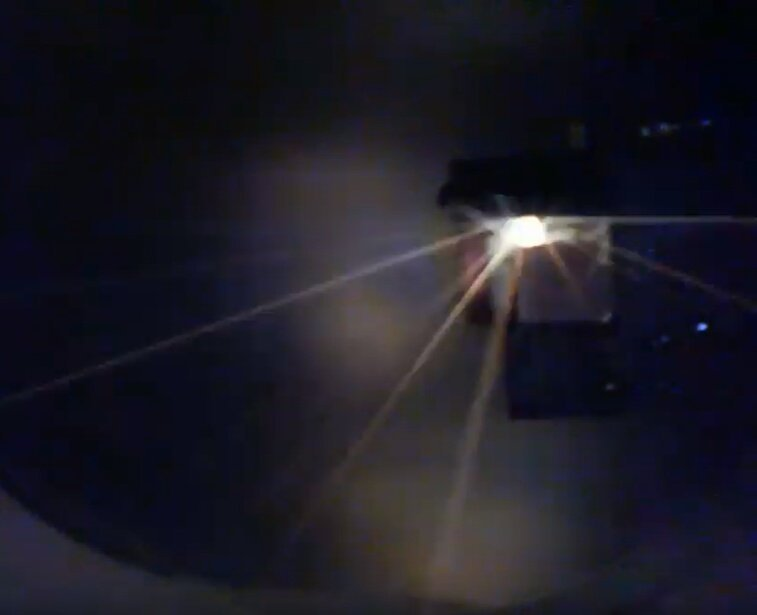
\includegraphics[width=10cm,keepaspectratio]{cap-failure.jpg}
\caption{Video frame from test chamber at the moment of failure}
\label{failure}
\end{figure}

Antikernel Labs performed a best-effort analysis at no cost in order to support the open-hardware nature of AIS's work.

This document is licensed under Creative Commons Attribution-NonCommercial-NoDerivatives 4.0 International.

\pagebreak
\section{Specimen Overview}

Two Kemet C4540H683KGGWCT050 capacitors were provided by AIS: the failed part, as well as an identical undamaged
capacitor (Fig. \ref{overview}) removed from the failed board to be used for process development and testing.

The capacitor is a 11.4 x 10.2 x 2.7 mm multi-layer ceramic capacitor (MLCC) using C0G-type dielectric, with a nominal
capacitance of 68 nF and a 2 kV maximum voltage rating. It is intended for high voltage pulsed discharge applications.

\begin{figure}[h]
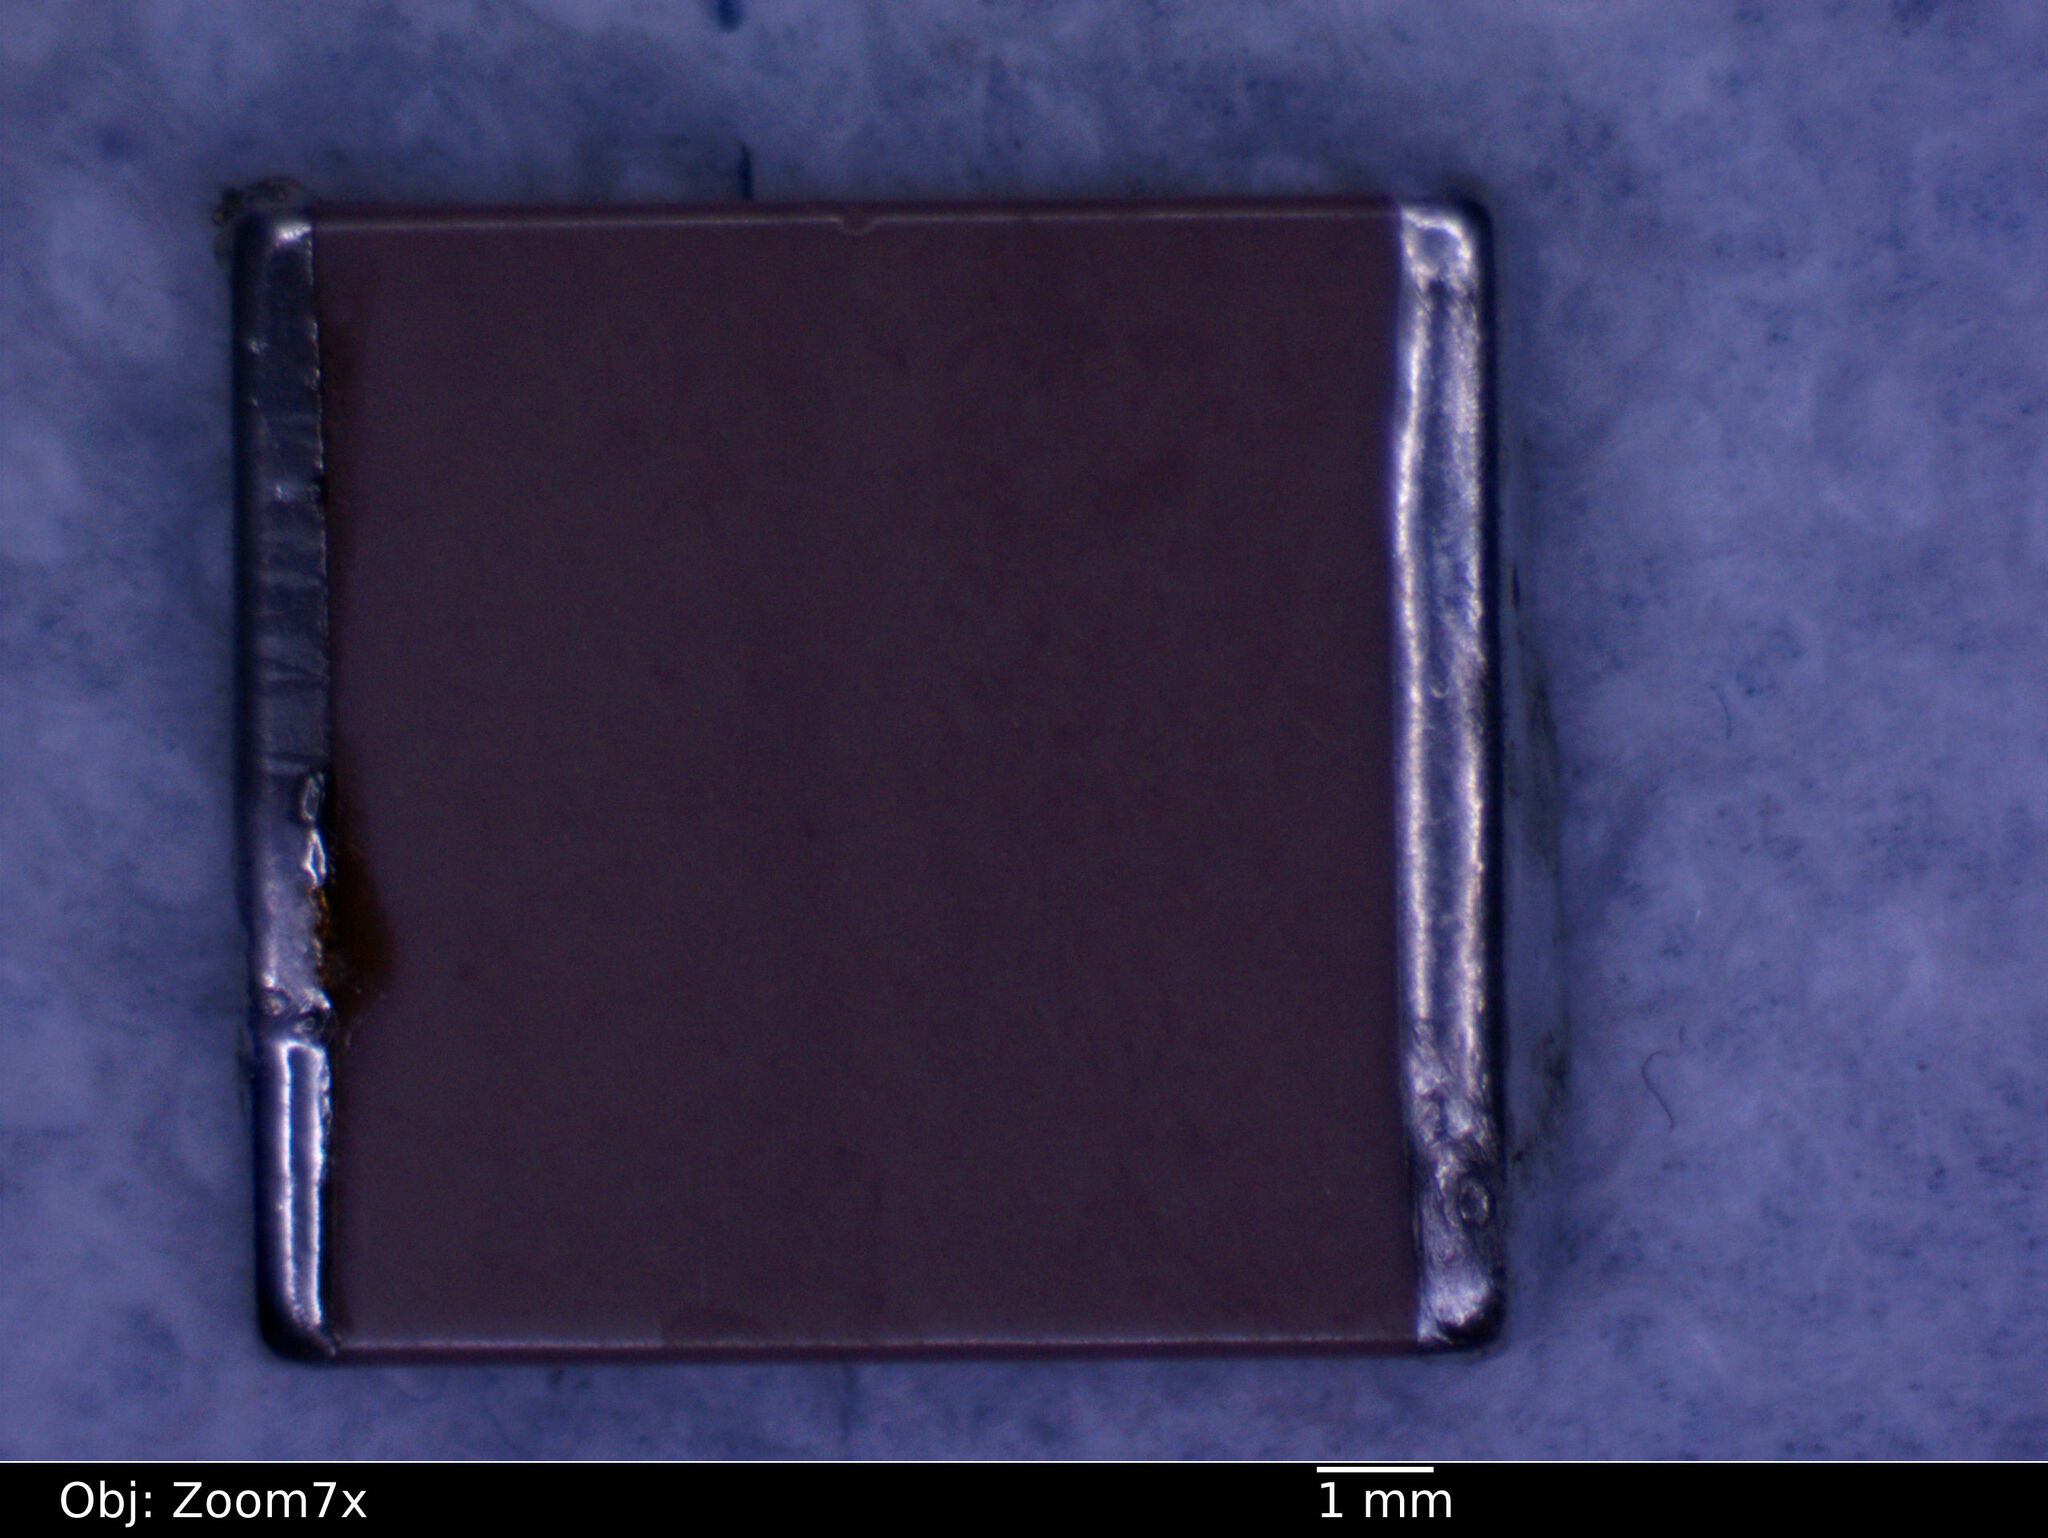
\includegraphics[width=10cm,keepaspectratio]{01-goodcap-top_annotated.jpg}
\caption{Top view of undamaged capacitor}
\label{overview}
\end{figure}

\pagebreak
\section{Analysis}

\subsection{Overview}

Preliminary optical imaging of the failed side of the capacitor (Fig. \ref{fail-overview}, Fig. \ref{fail-closeup})
showed a cratered region with long cracks radiating lengthwise down the capacitor body.

\begin{figure}[h]
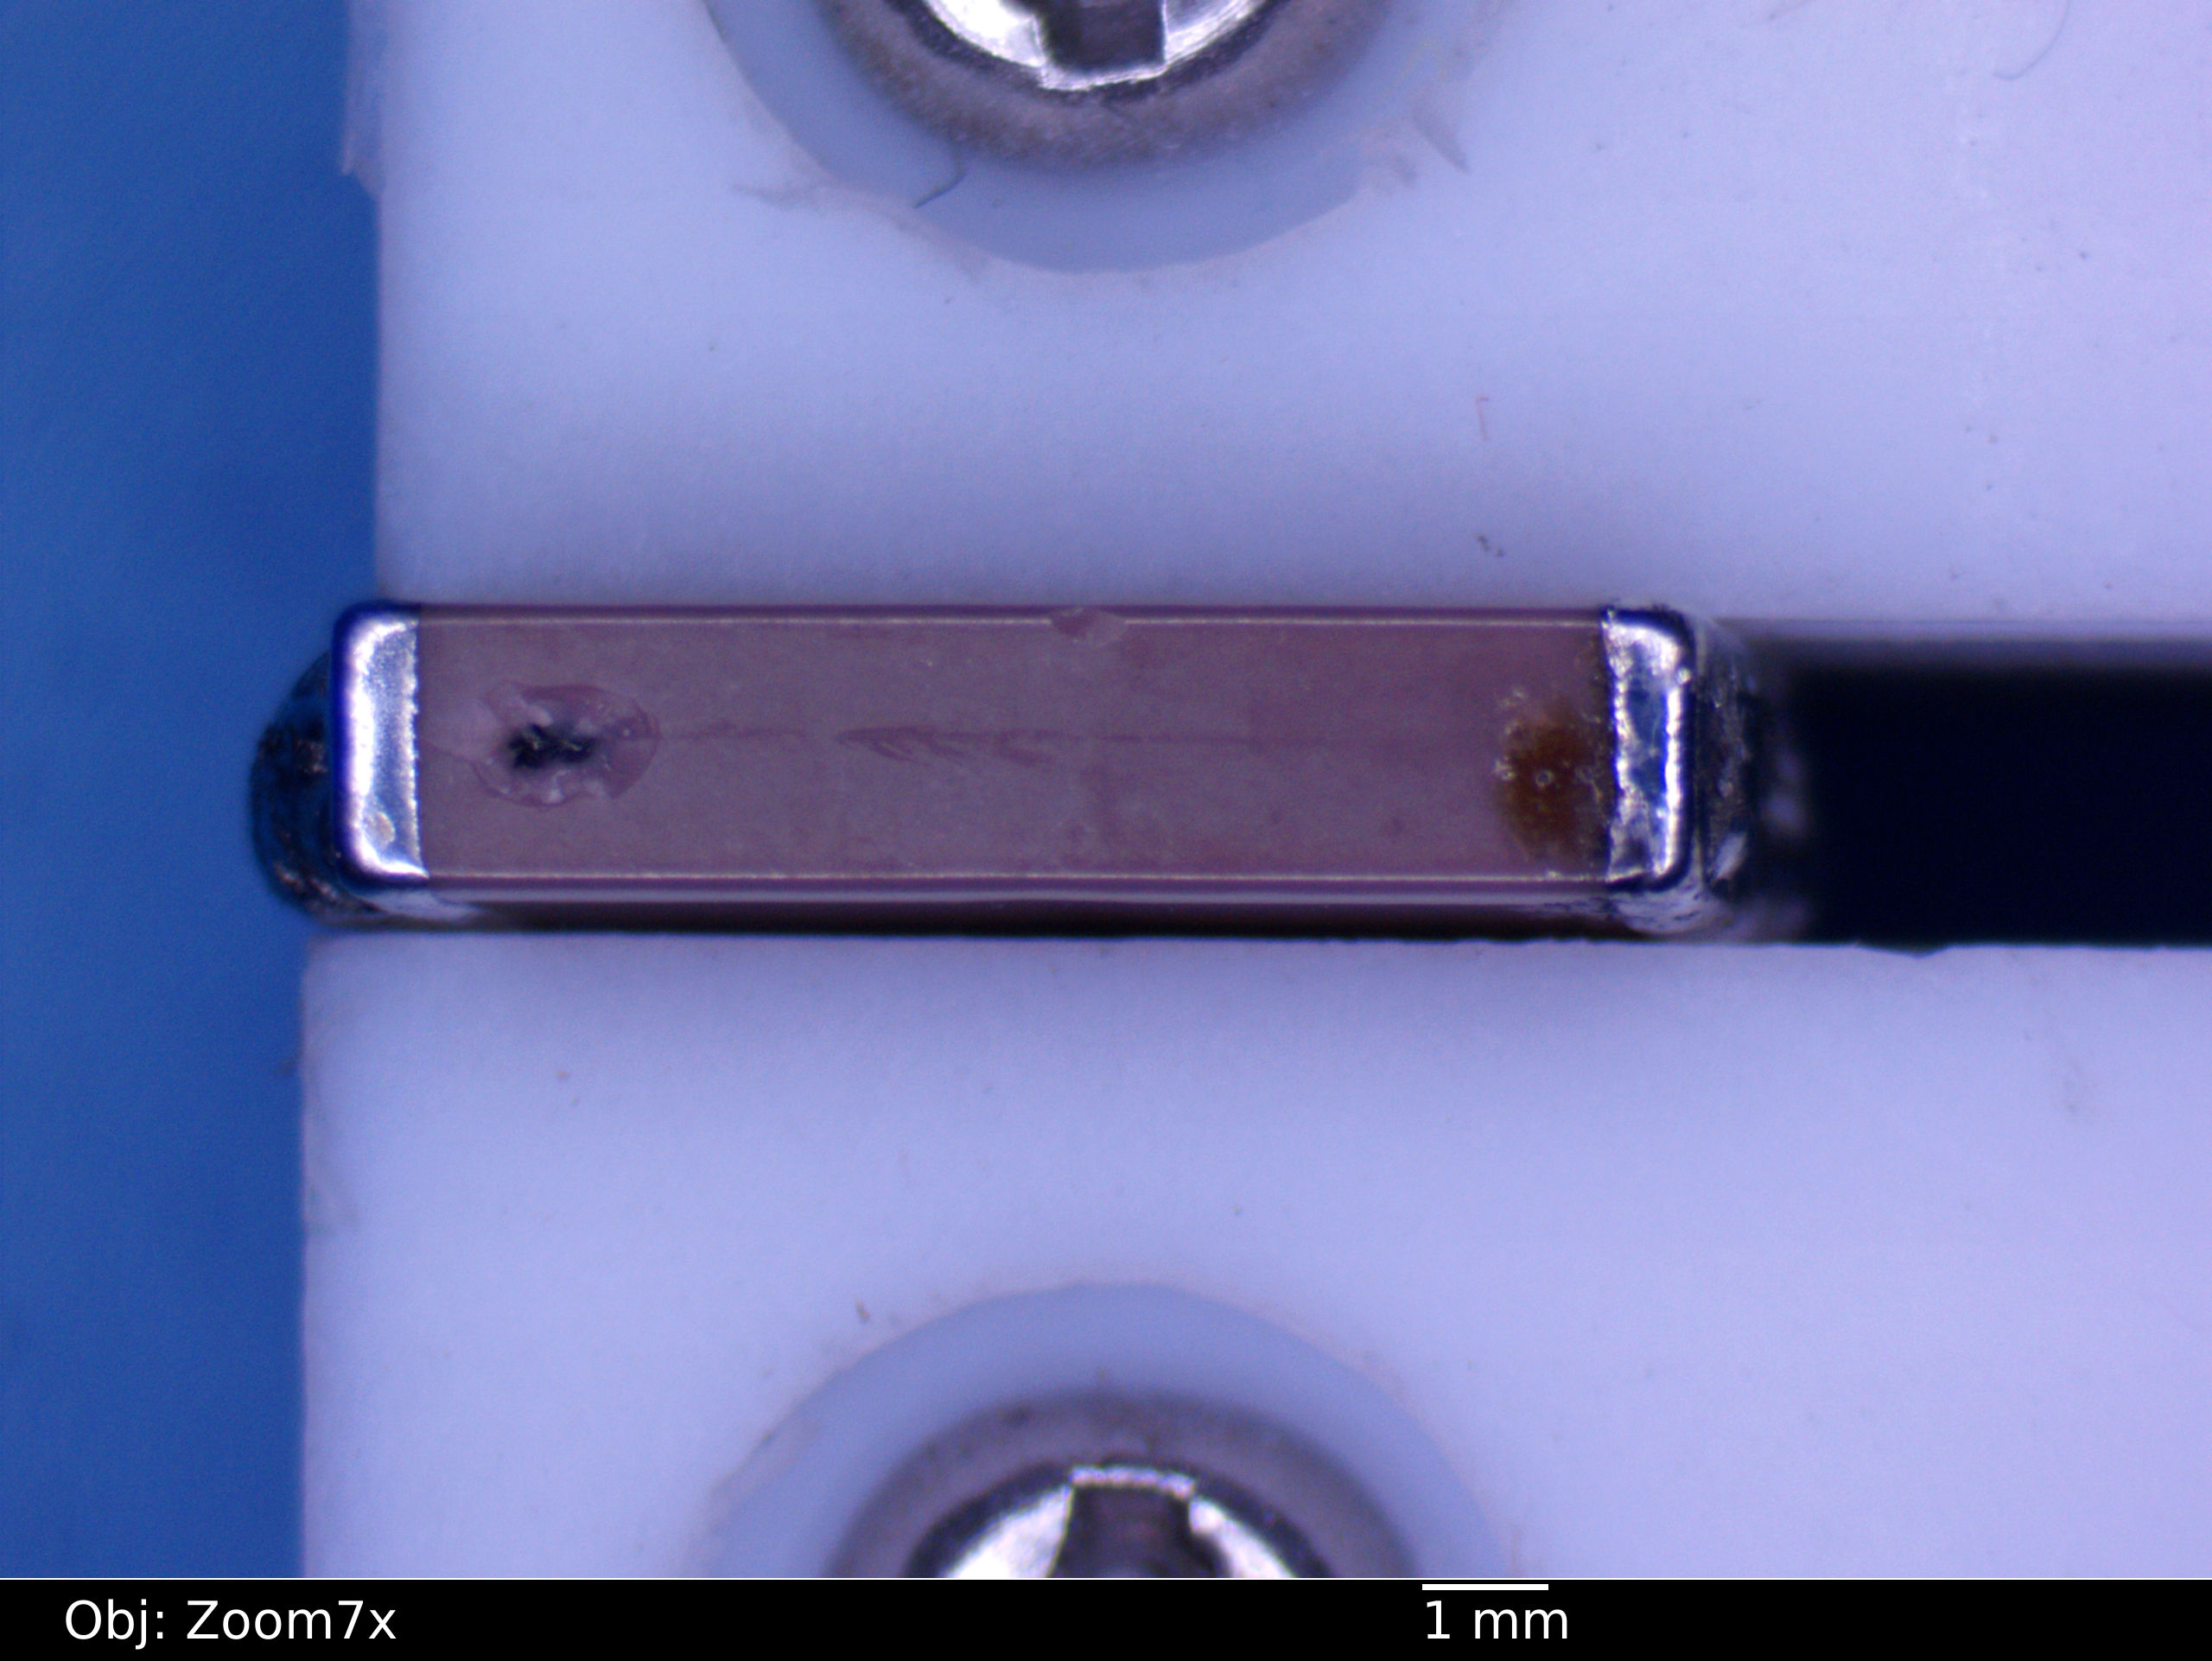
\includegraphics[width=8cm,keepaspectratio]{02-badcap-side_annotated.jpg}
\caption{Overview of failure site}
\label{fail-overview}
\end{figure}

\begin{figure}[h]
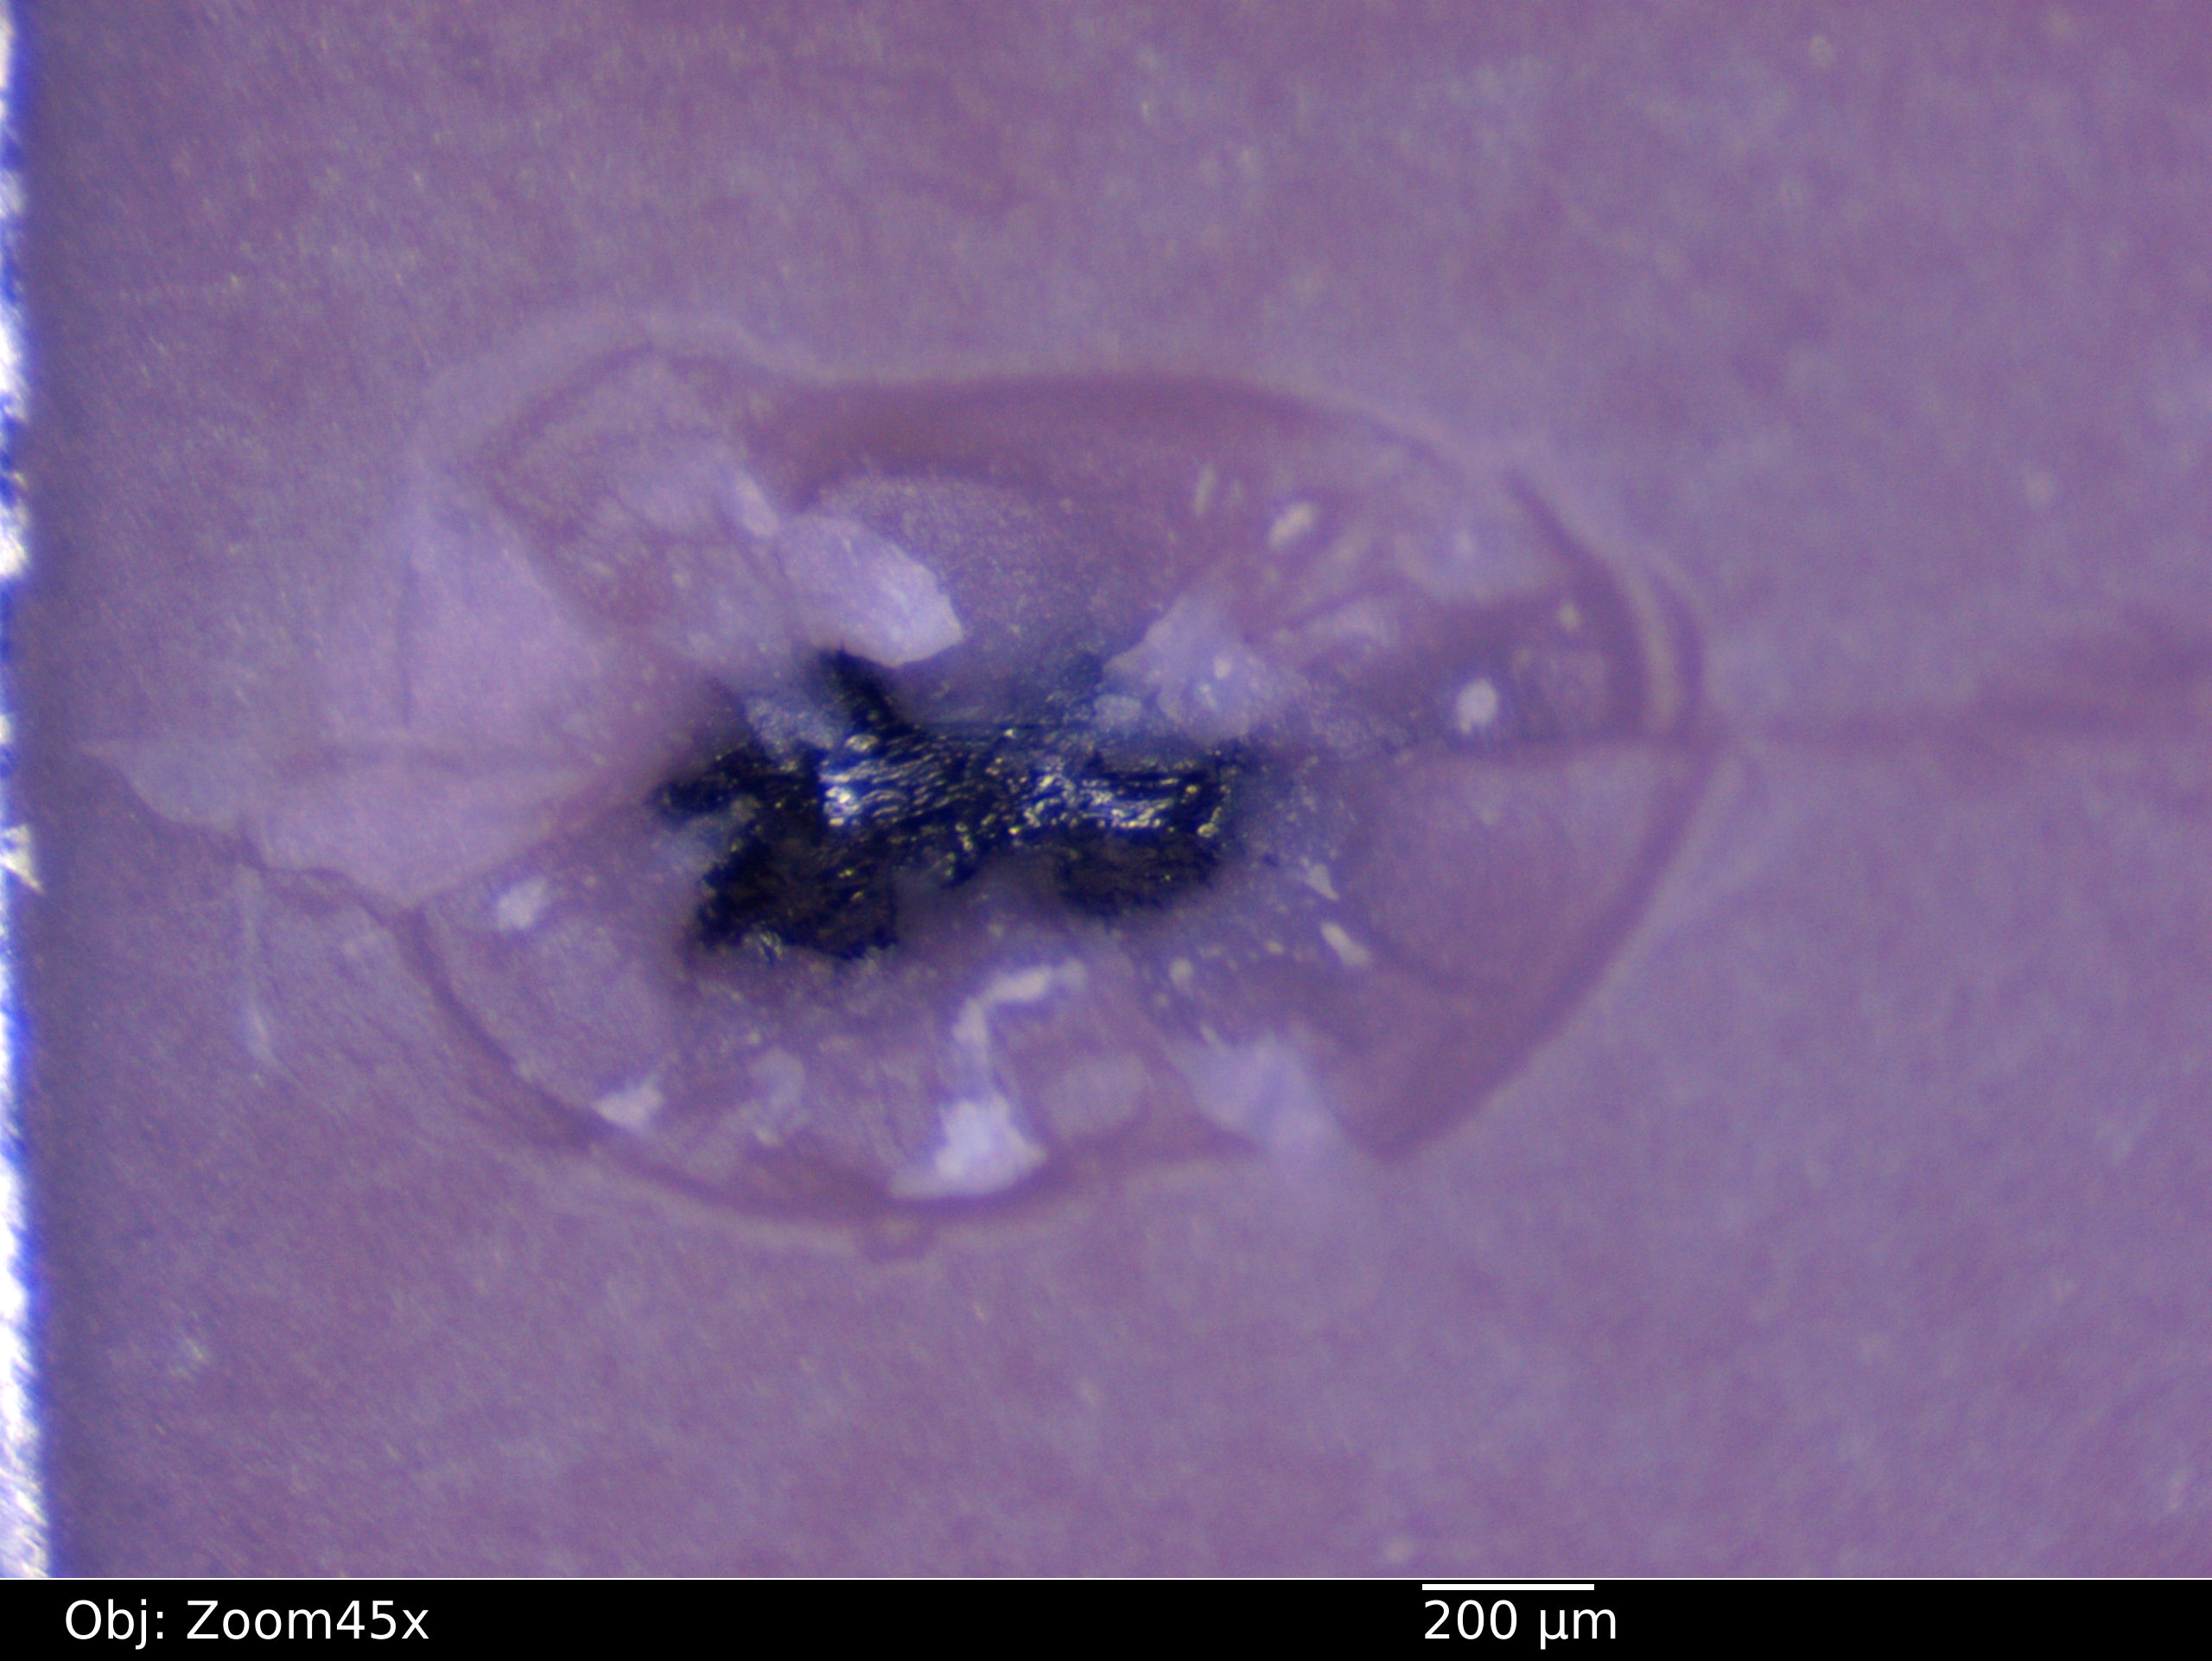
\includegraphics[width=8cm,keepaspectratio]{03-badcap-side_annotated.jpg}
\caption{Closeup of failure site}
\label{fail-closeup}
\end{figure}

\FloatBarrier

\subsection{Slice 1}

The large size of the capacitor presented some unique challenges for analysis, since it was too large to fit edgewise
into most standard embedding molds.

Experimentation with using power tools to cut down the test capacitor led to excessive cracking, so bulk material
removal on the failed specimen was performed by hand sanding using P150 and P220 $Al_2O_3$ sandpaper.

The sample was embedded in epoxy resin (AA-Bond F110, Atom Adhesives, Fig.\ref{section-overview}) and ground with P220
$Al_2O_3$ sandpaper until the solder and copper terminal were removed. A preliminary cross section immediately past the
terminal surface (slightly to the left of the green bar in Fig. \ref{section-plane}) was polished with P500, P1200,
P2000, P3000, P5000, P8000, and P10000 $SiC$ sandpaper, then lapped with 300 nm $Al_2O_3$ to produce an optically flat
surface

\begin{figure}[h]
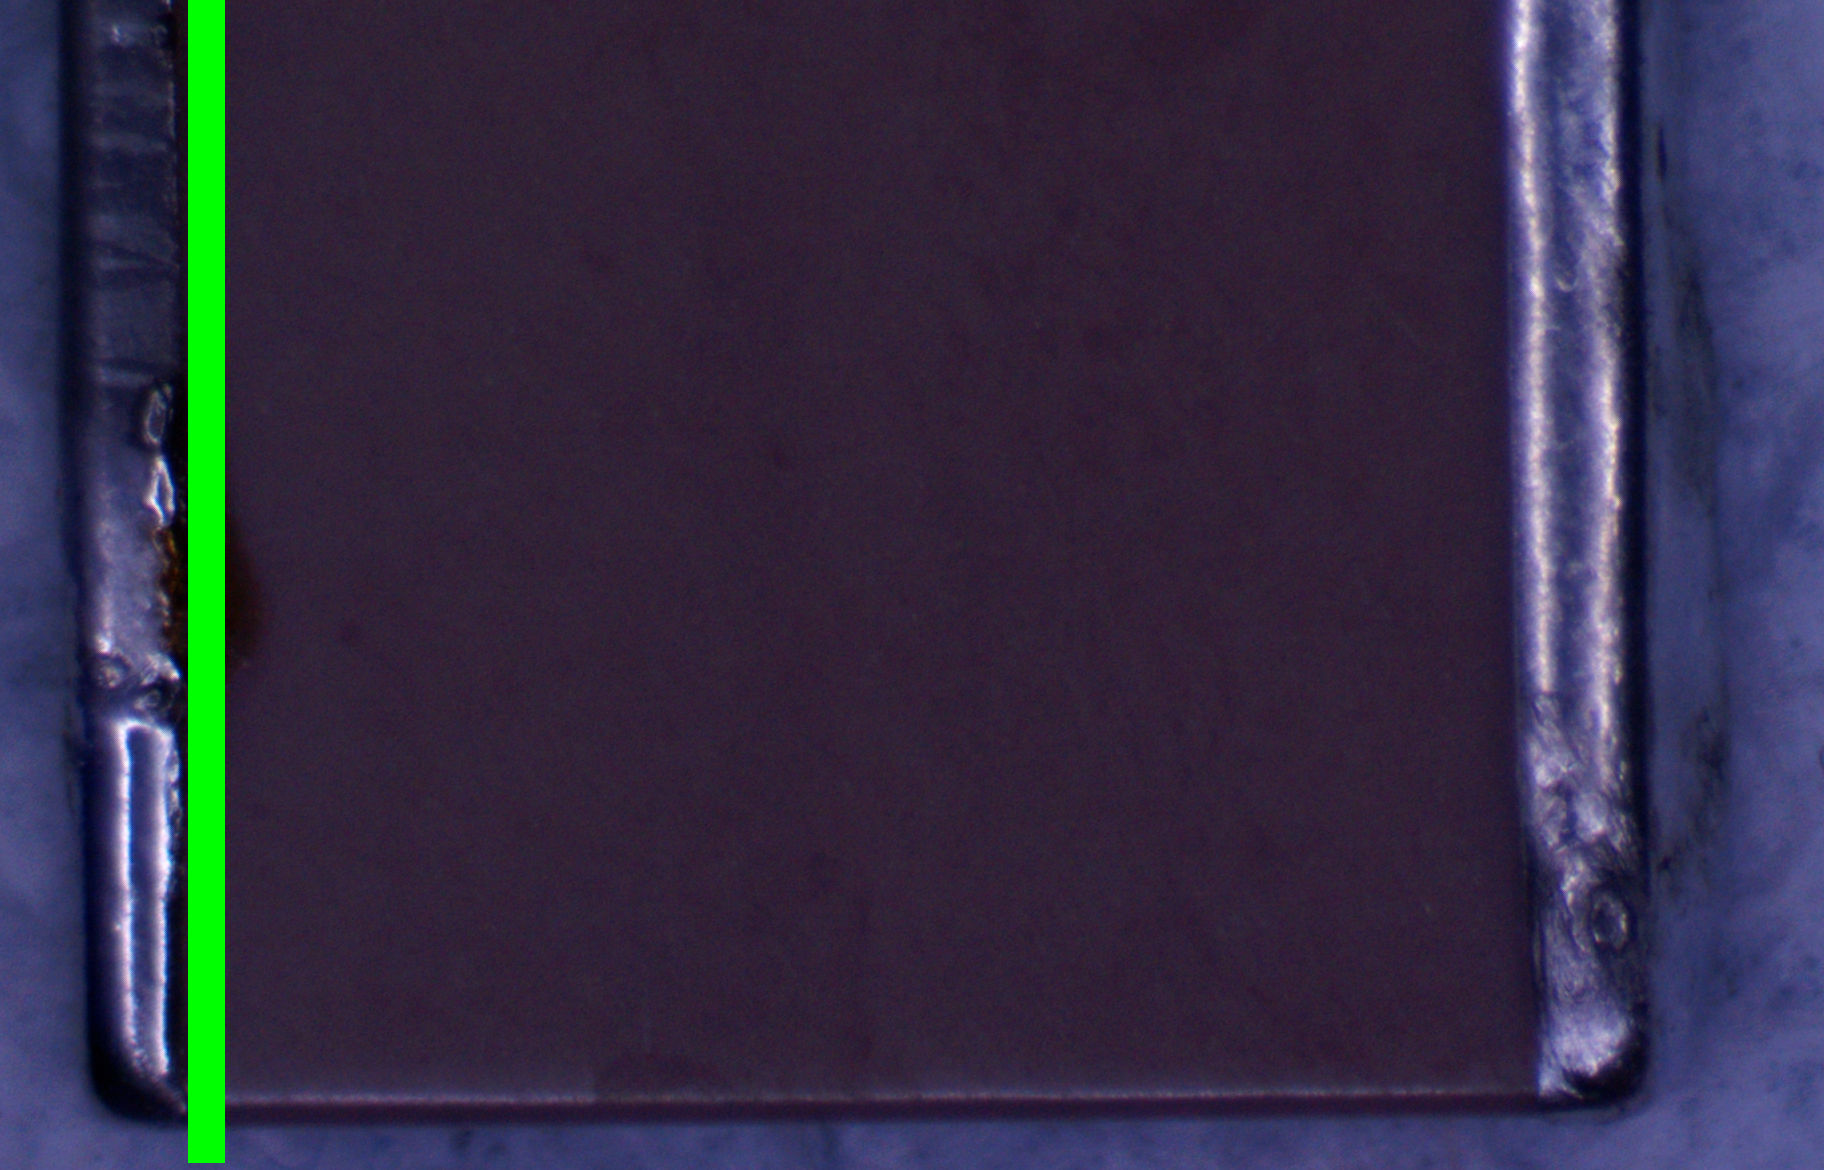
\includegraphics[width=10cm,keepaspectratio]{section-plane.jpg}
\caption{Cross sectioning plane orientation relative to capacitor body}
\label{section-plane}
\end{figure}

\begin{figure}[h]
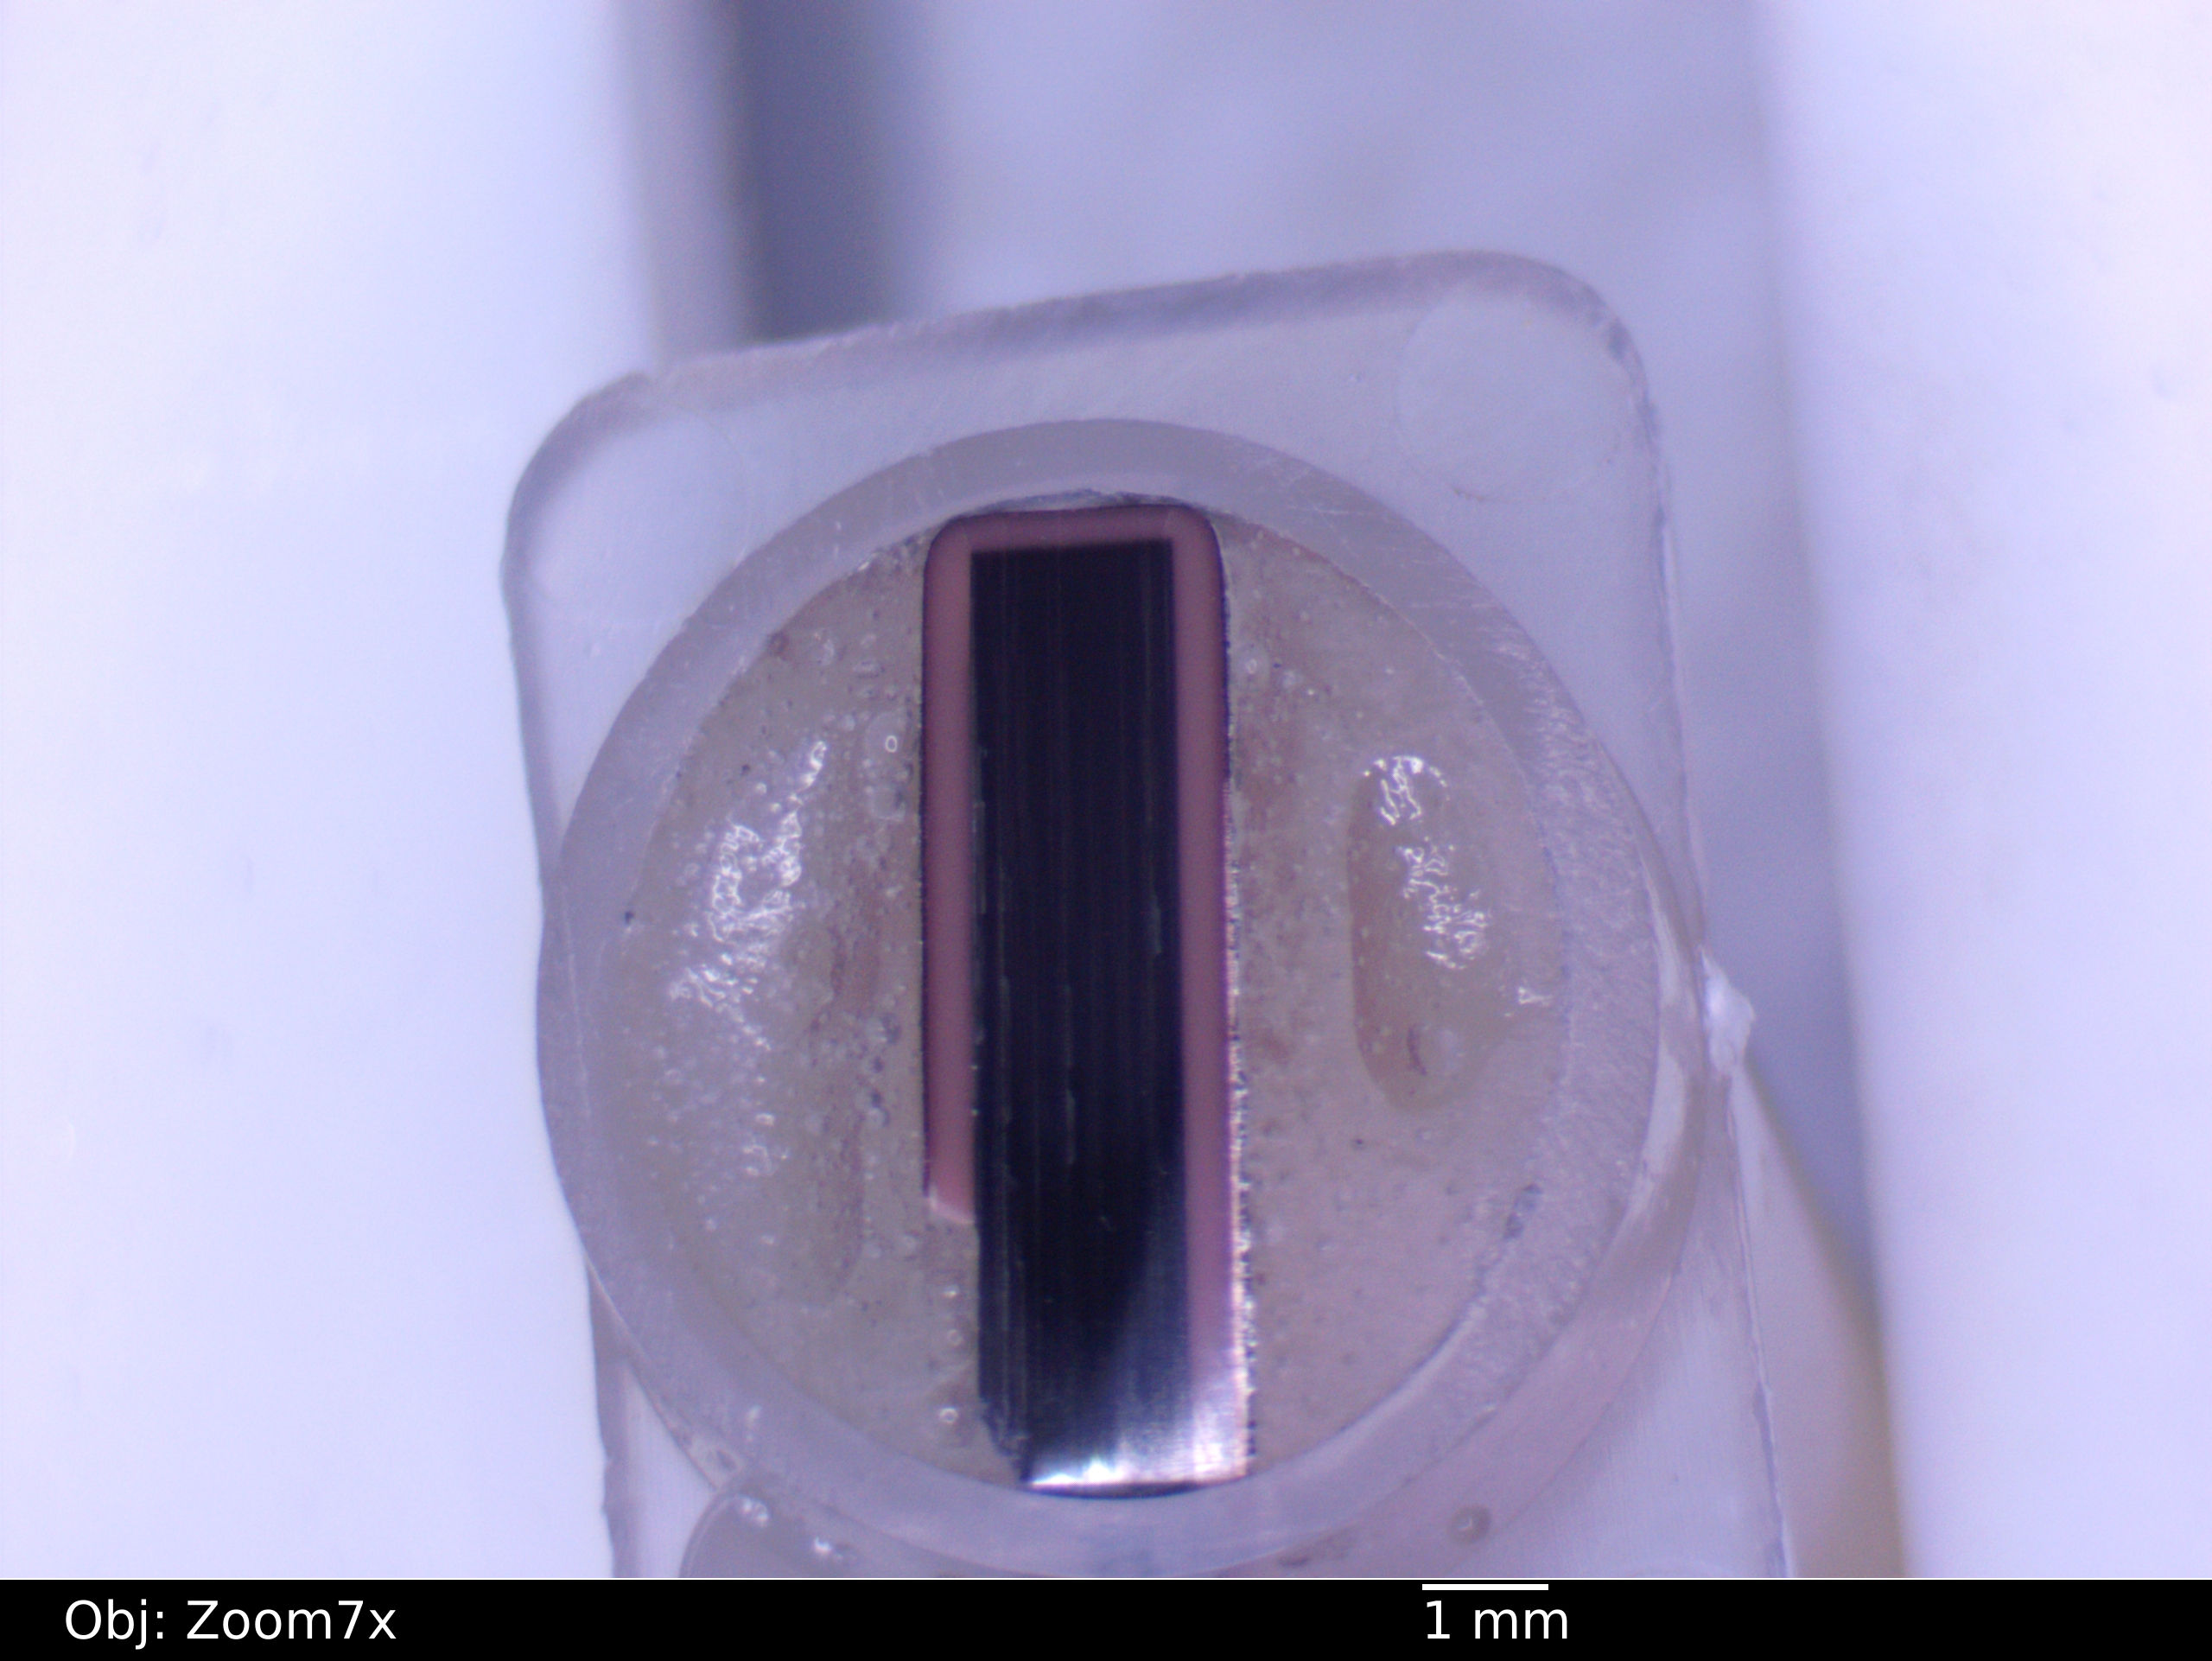
\includegraphics[width=11cm,keepaspectratio]{07-section1-7x_annotated.jpg}
\caption{Cross section overview}
\label{section-overview}
\end{figure}

This section showed a stack of 64 plates (Fig. \ref{section-plates}) with a total thickness of $1610 \mu m$, separated
from the top and bottom component faces by $355 \mu m$ of ceramic shell. Shell thickness from the edges of the plate
stack to the sides of the capacitor was $245 \mu m$.

Plates were approximately $1.4 \mu m$ thick, separated by $25 \mu m$ of the C0G dielectric. Since this section was
taken immediately adjacent to a terminal, only plates connecting to this terminal were visible.

\begin{figure}[h]
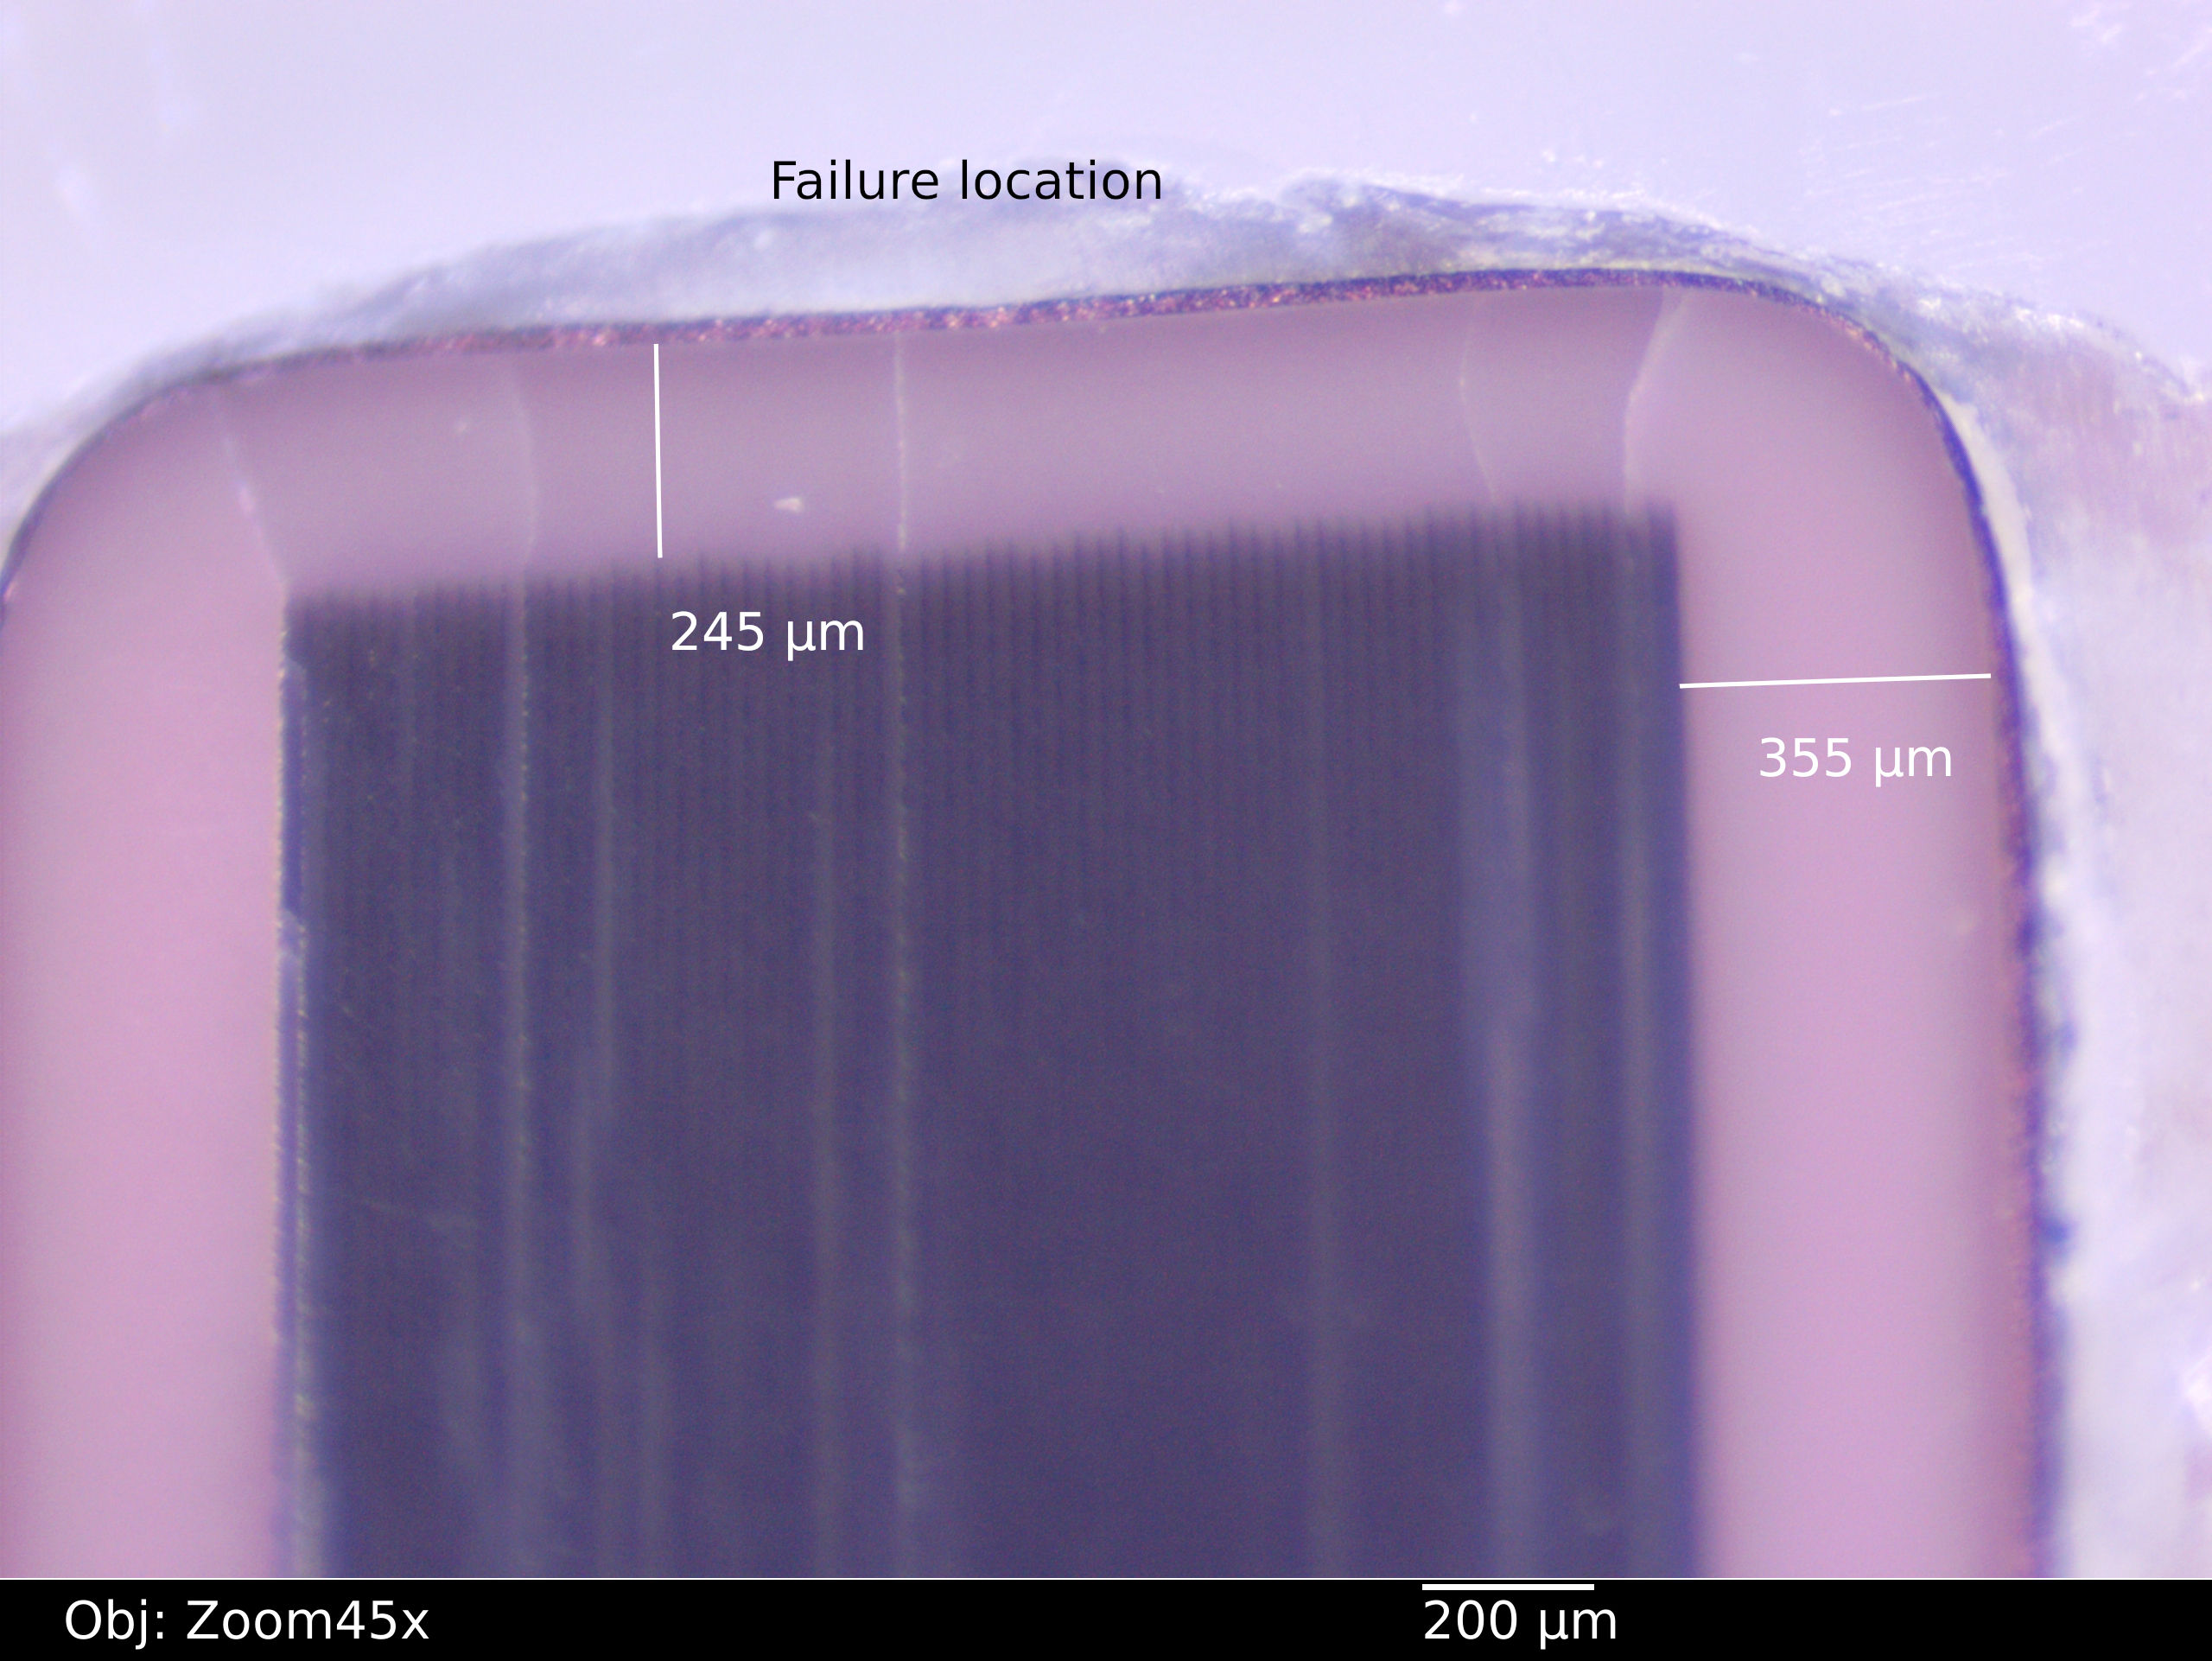
\includegraphics[width=11cm,keepaspectratio]{06-section1-45x_annotated2.jpg}
\caption{Cross section showing dielectric thicknesses and locations of some cracks}
\label{section-plates}
\end{figure}

\begin{figure}[h]
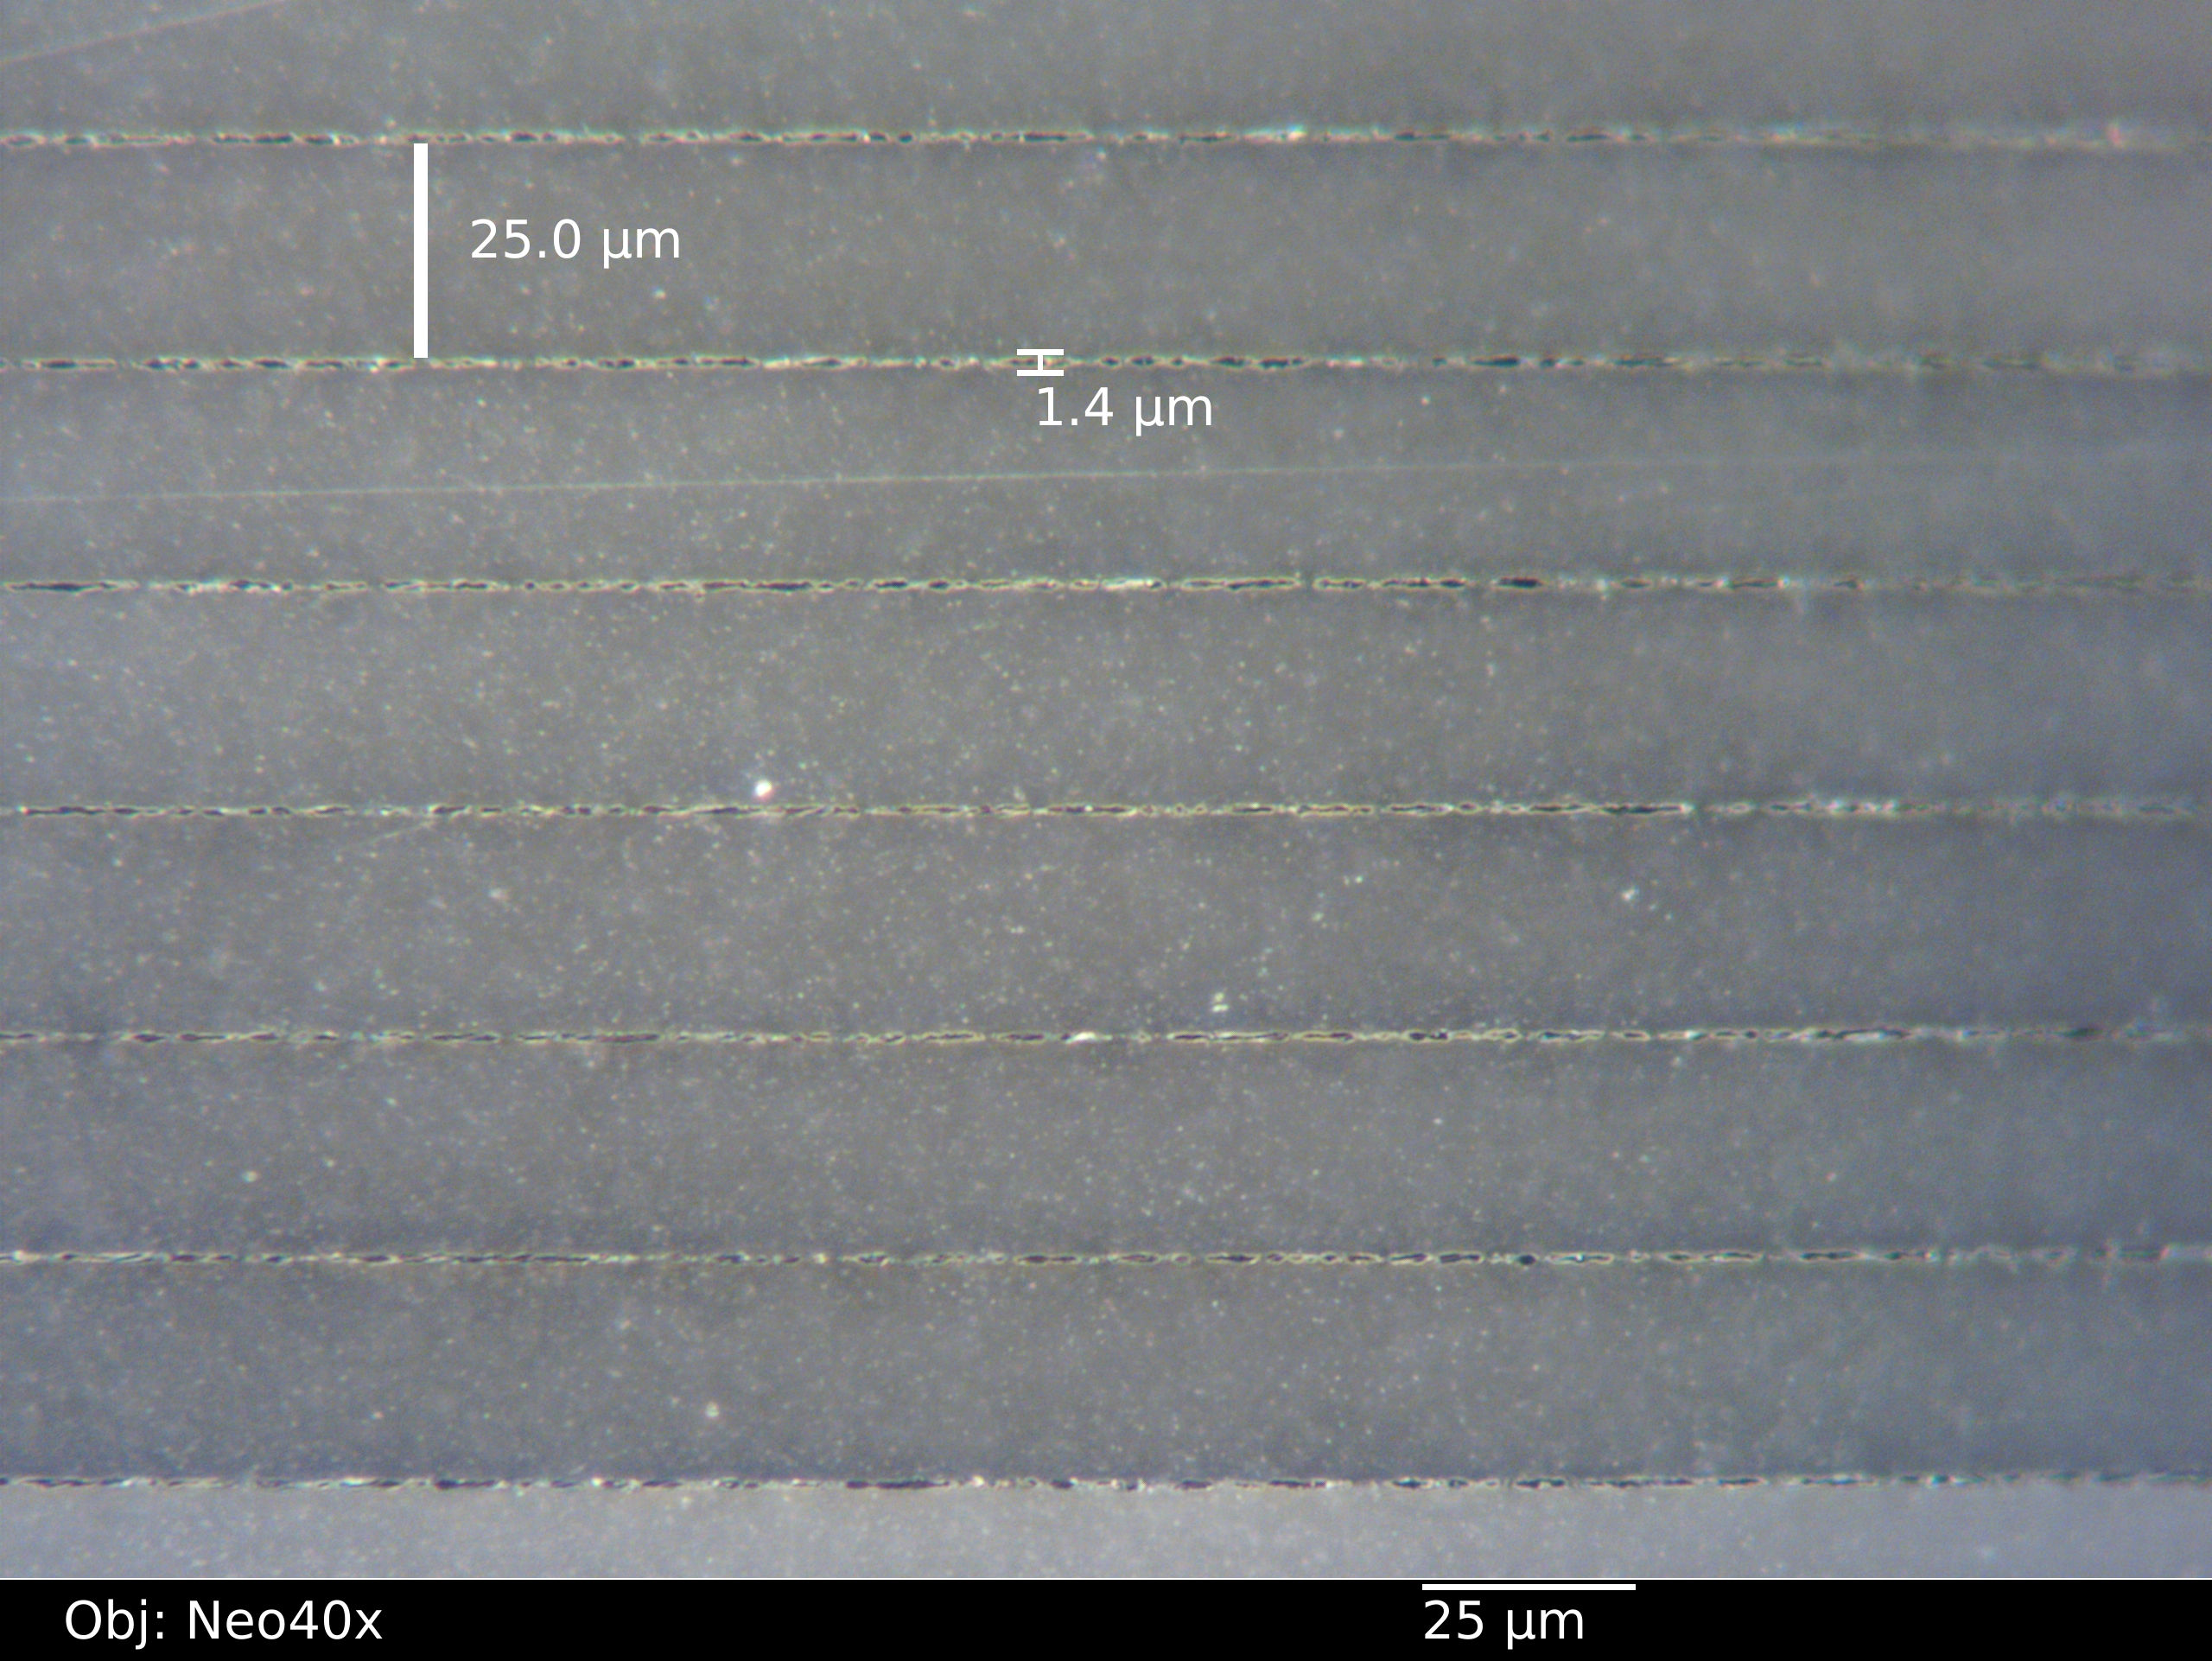
\includegraphics[width=11cm,keepaspectratio]{section1_09_df_neo40x_annotated2.jpg}
\caption{Thickness and spacing of capacitor plates in terminal area}
\label{plate-dimensions}
\end{figure}

Numerous cracks in the dielectric (Fig. \ref{cracks1}, Fig. \ref{cracks2}) were visible on the side of the capacitor
closest to the failure site. These are likely the result of thermal stress during overheating at the moment of failure.

\begin{figure}[h]
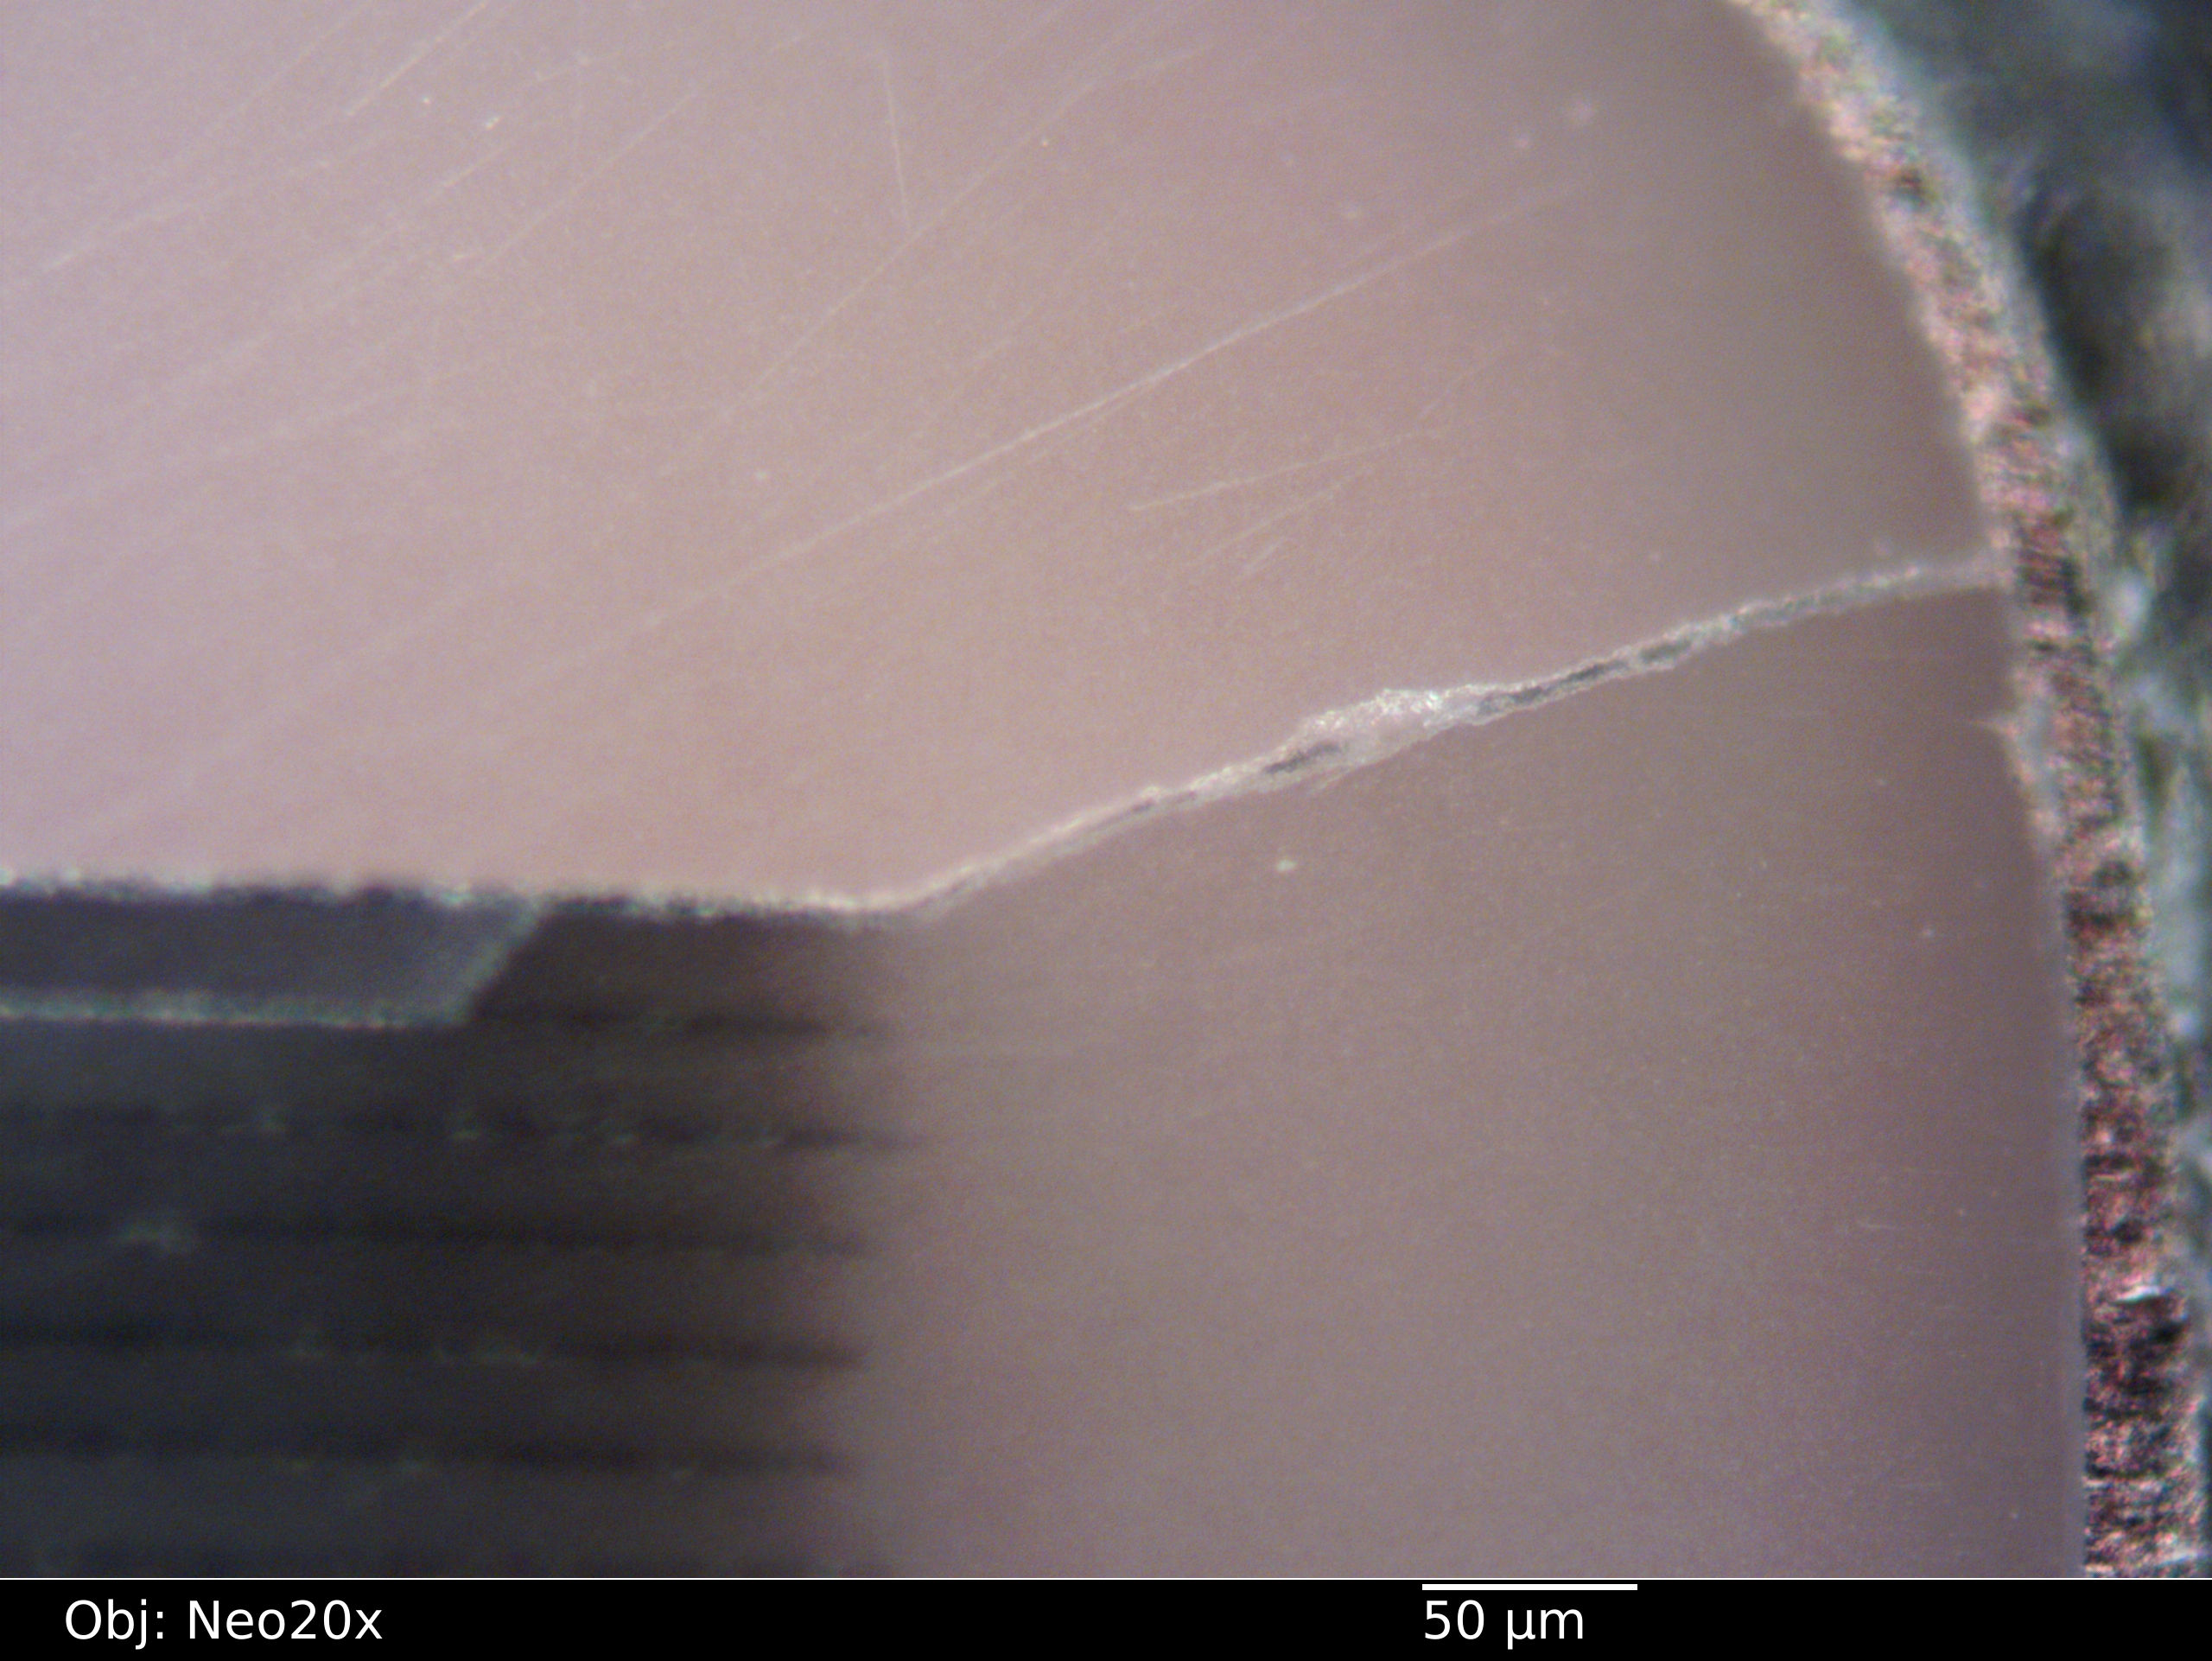
\includegraphics[width=11cm,keepaspectratio]{section1_05_df_neo20x_annotated.jpg}
\caption{Crack at right corner of topmost capacitor plate.}
\label{cracks1}
\end{figure}

\begin{figure}[h]
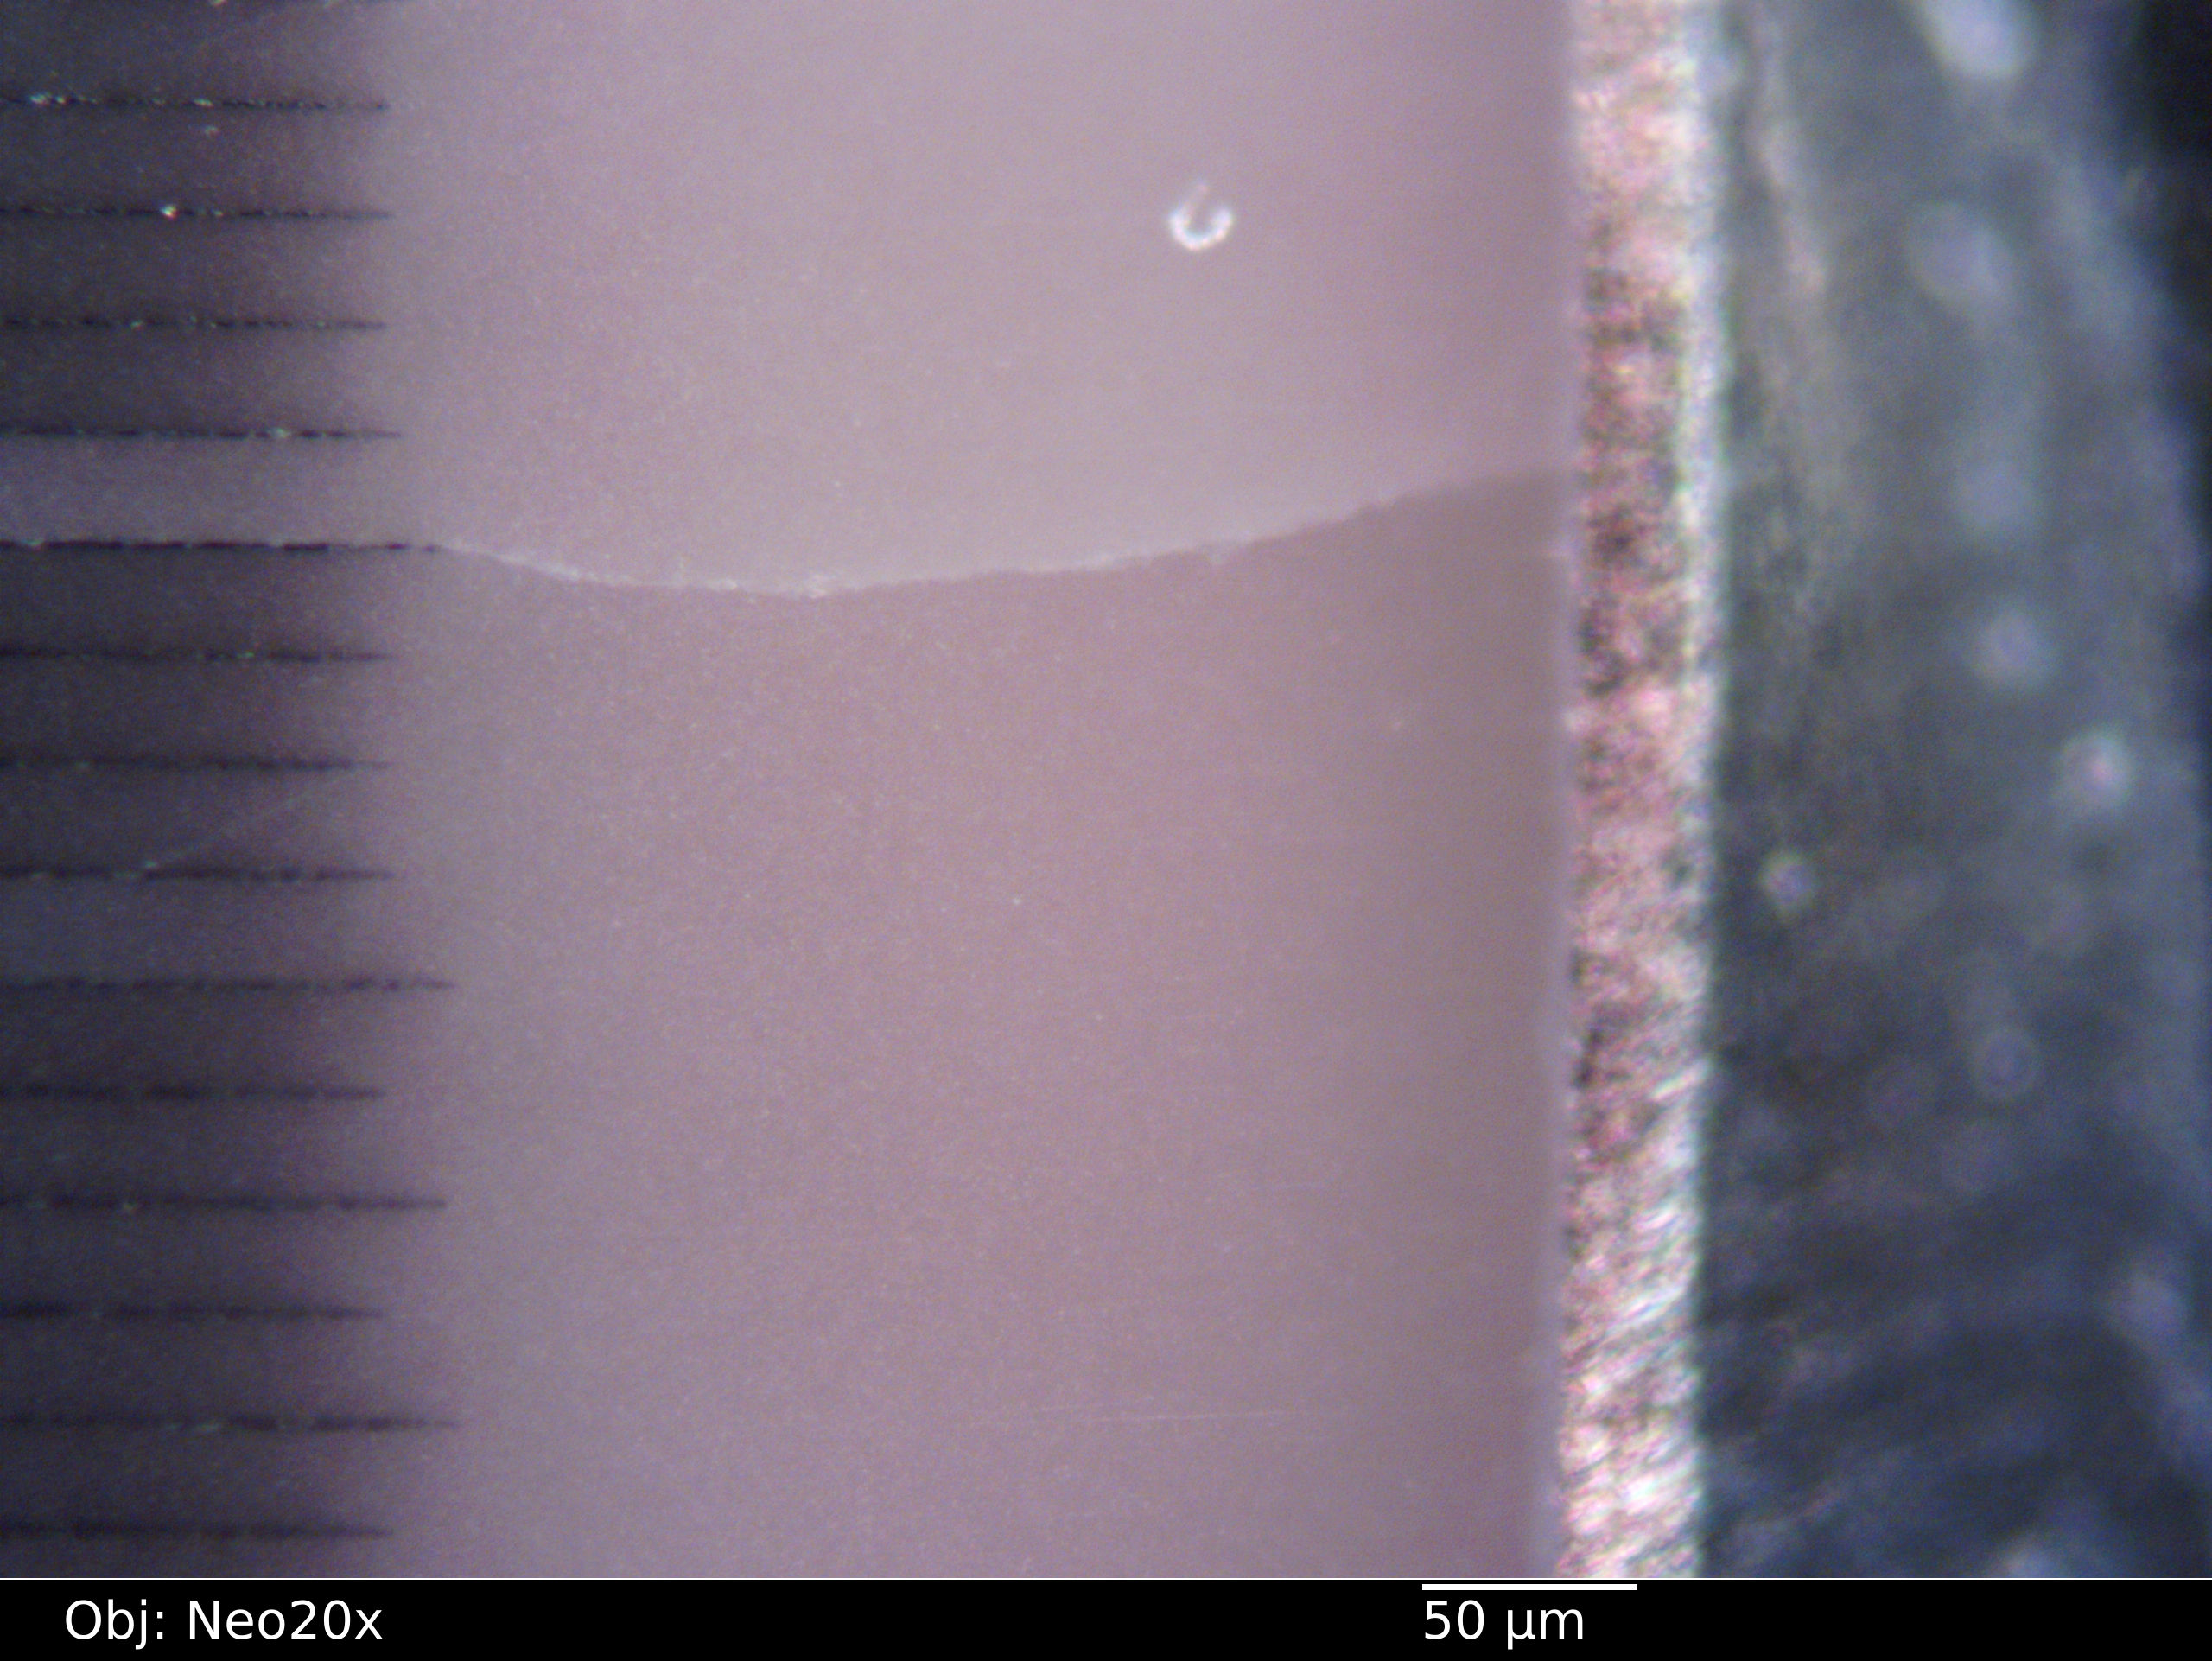
\includegraphics[width=11cm,keepaspectratio]{section1_06_df_neo20x_annotated.jpg}
\caption{Crack at right side of capacitor}
\label{cracks2}
\end{figure}

\FloatBarrier

\subsection{Slice 2}

The sample was ground down by $100 \mu m$ and polished using the same procedure as the previous section. The same five
large cracks seen in the first section were visible here (Fig. \ref{section2_1}), propagating from the affected plates
to the side of the component. This delamination extended a significant distance through the capacitor, however it was
difficult to identify an exact end point.

The 64 even and 63 odd plates (127 total, 126 gaps) were uniformly separated by $11.8 \mu m$ (Fig.
\ref{plate-geometry}) of C0G dielectric. Even numbered plates (connecting to the far terminal) were displaced to the
left by approximately $140 \mu m$ with respect to the odd numbered plates, however there was approximately
$\pm 10 \mu m$ of variability in exact horizontal position of each plate.

The center crack (closest to the actual blowout location) exhibited rounded fracture/spall patterns along it (Fig.
\ref{spalling}, \ref{spalling2}, \ref{spalling3}). Based on external examination (Fig. \ref{fail-overview}) this crack
appears to extend through most of the device. The damage appears to be more severe than the other cracks, which is
consistent with its location close to the externally visible failure.

\begin{figure}[h]
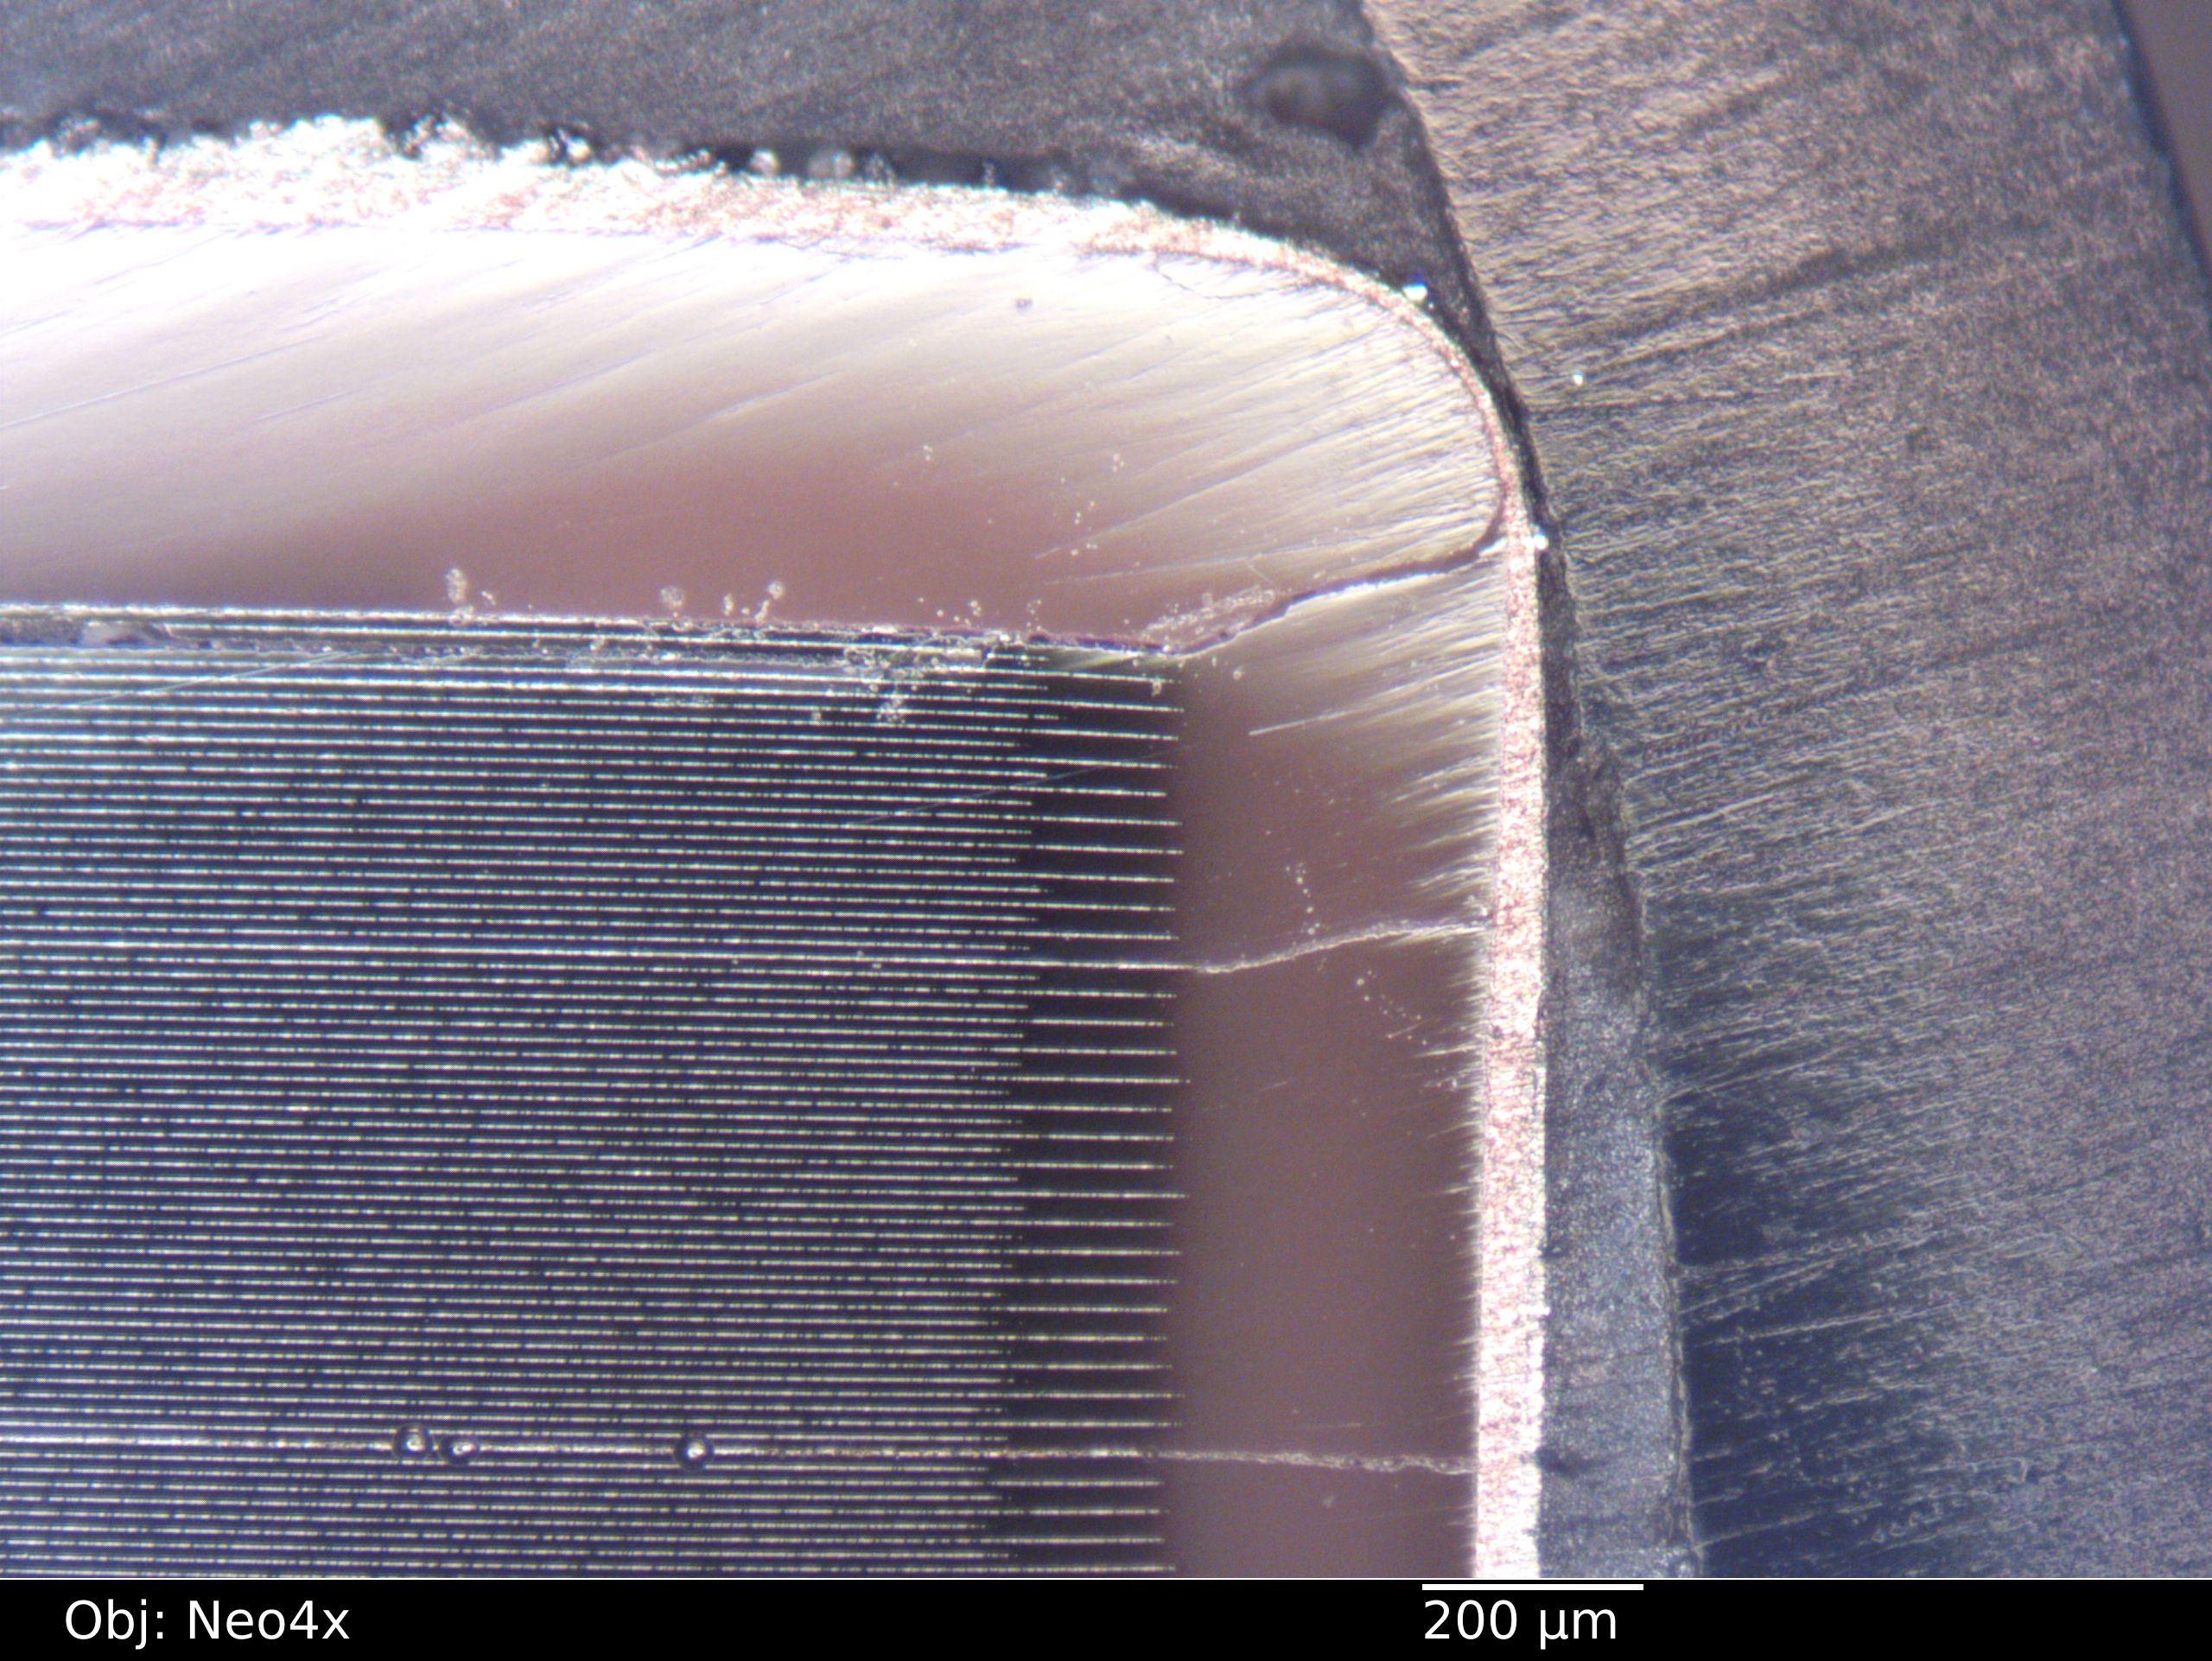
\includegraphics[width=14cm,keepaspectratio]{section2_02_df_neo4x_annotated.jpg}
\caption{Upper right corner of section 2}
\label{section2_1}
\end{figure}

\begin{figure}[h]
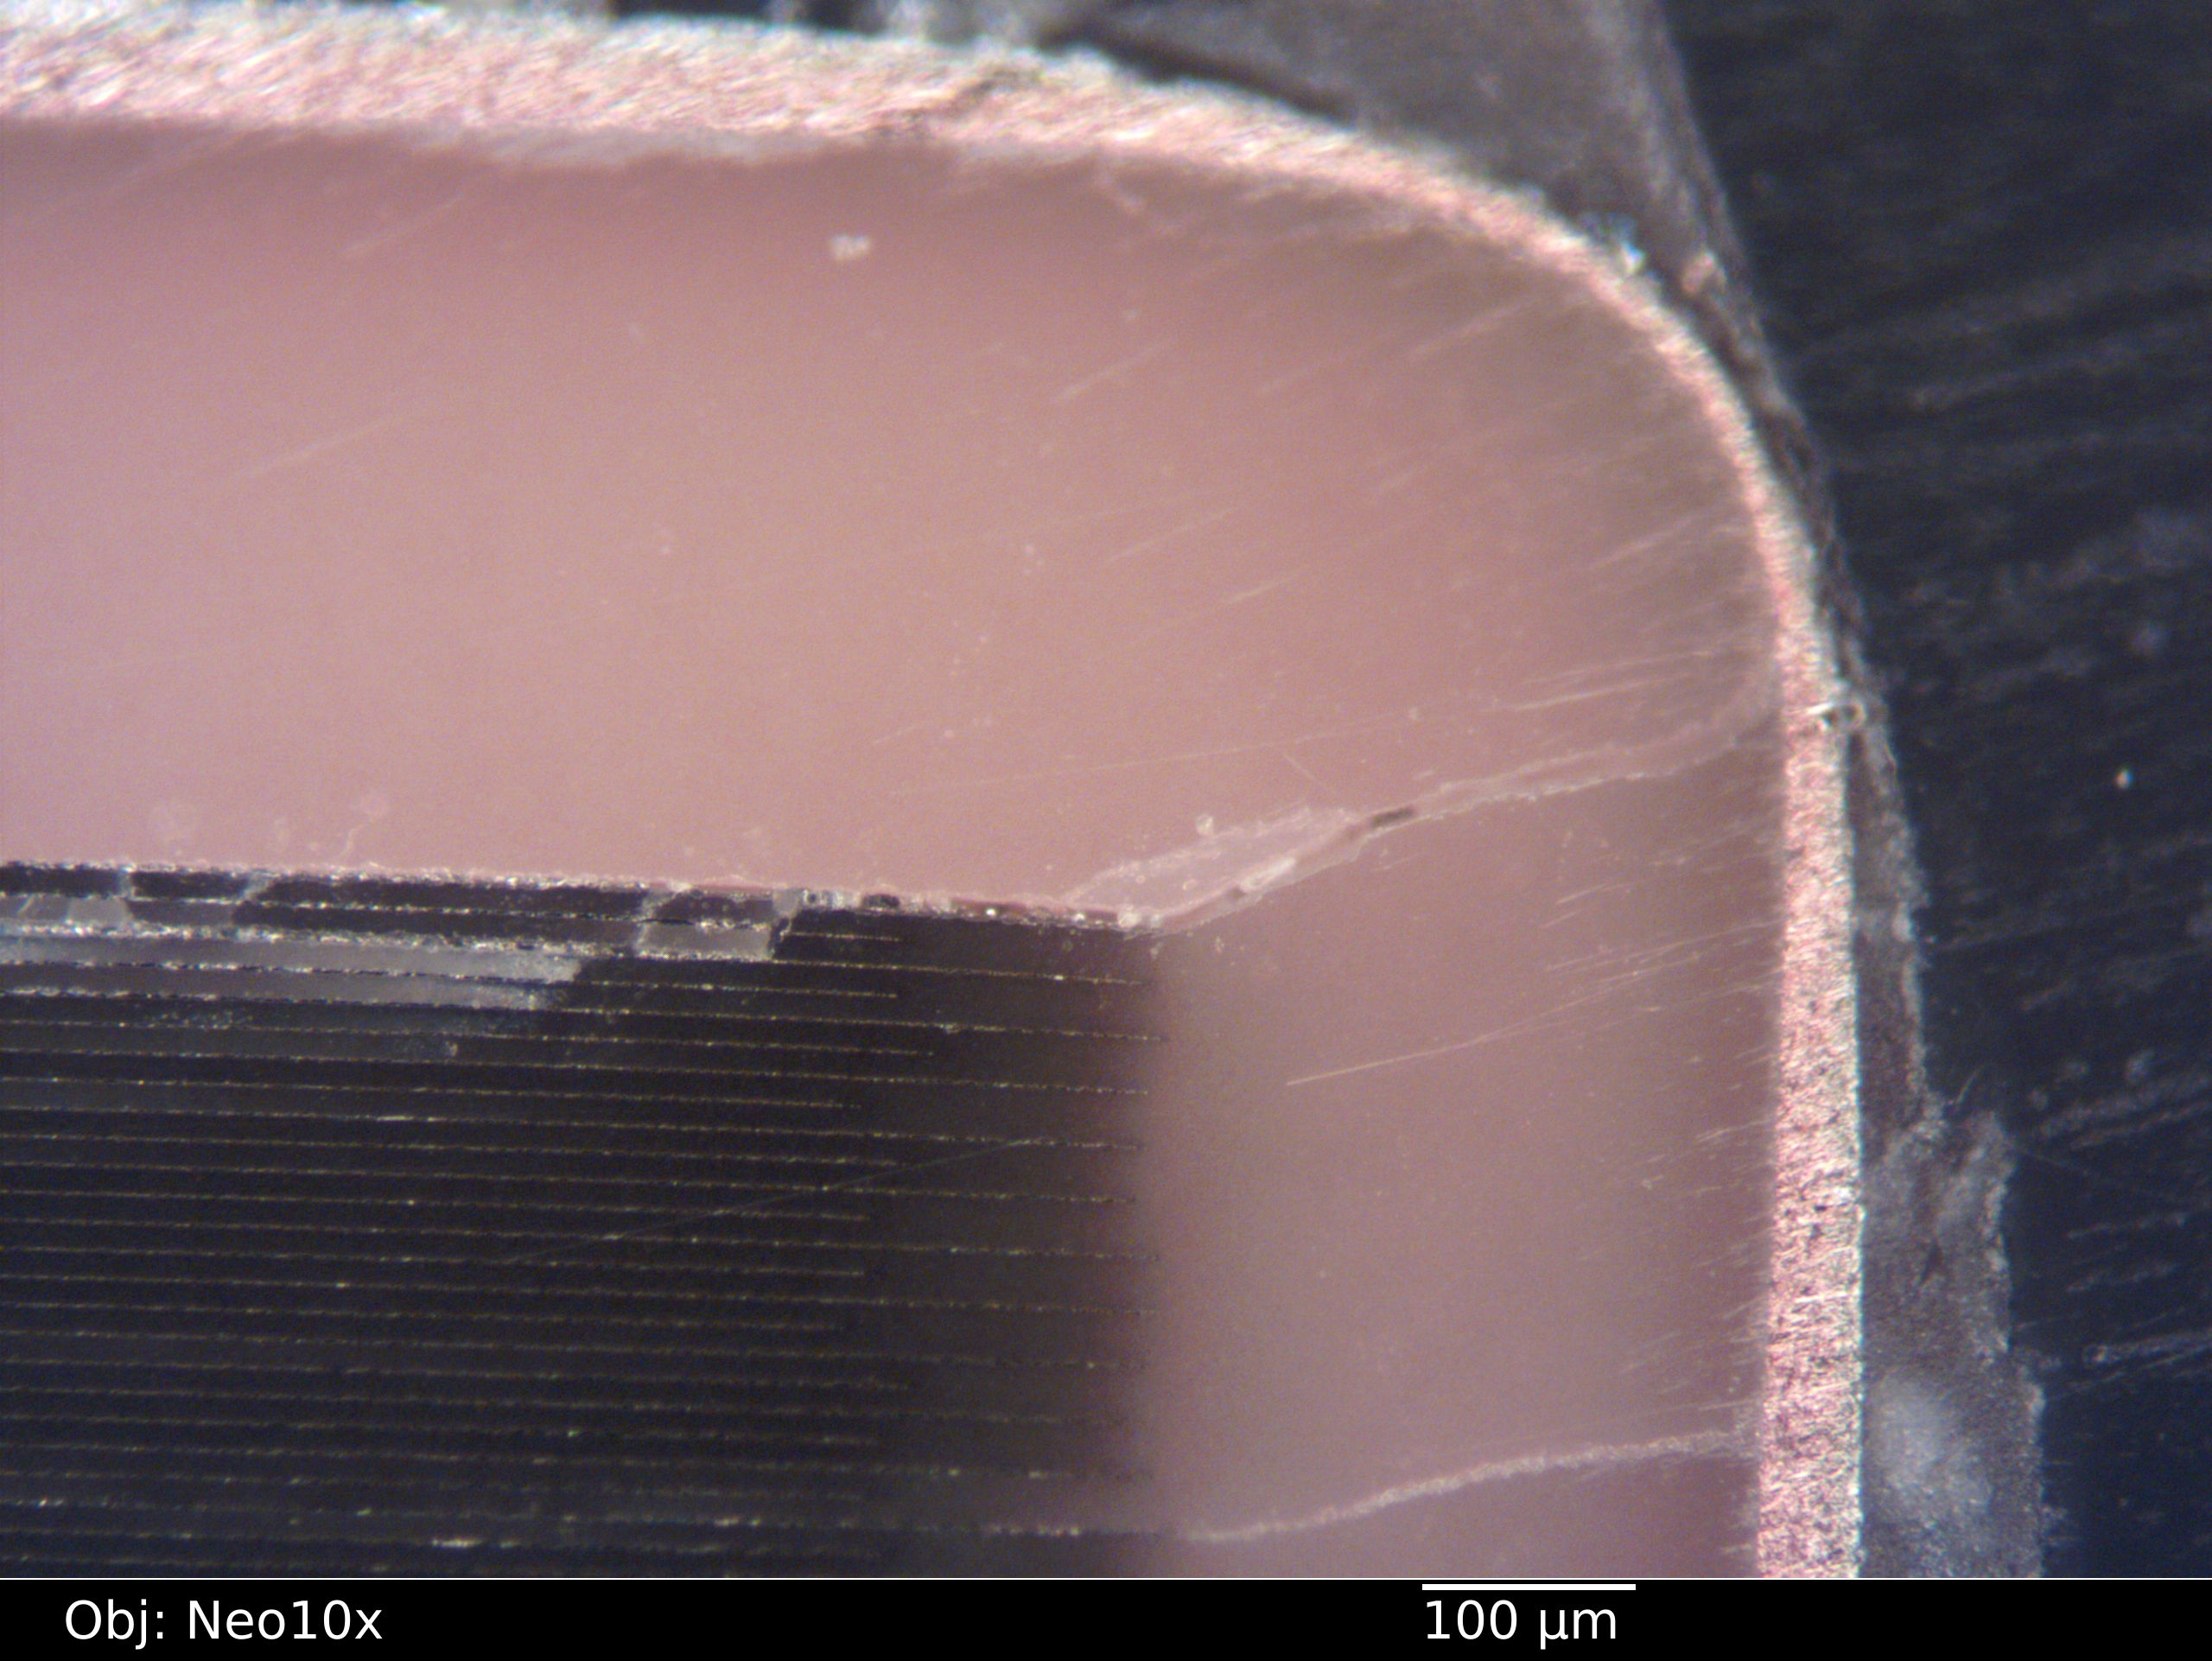
\includegraphics[width=11cm,keepaspectratio]{section2_03_df_neo10x_annotated.jpg}
\caption{Closeup of upper right corner}
\label{section2_2}
\end{figure}

\begin{figure}[h]
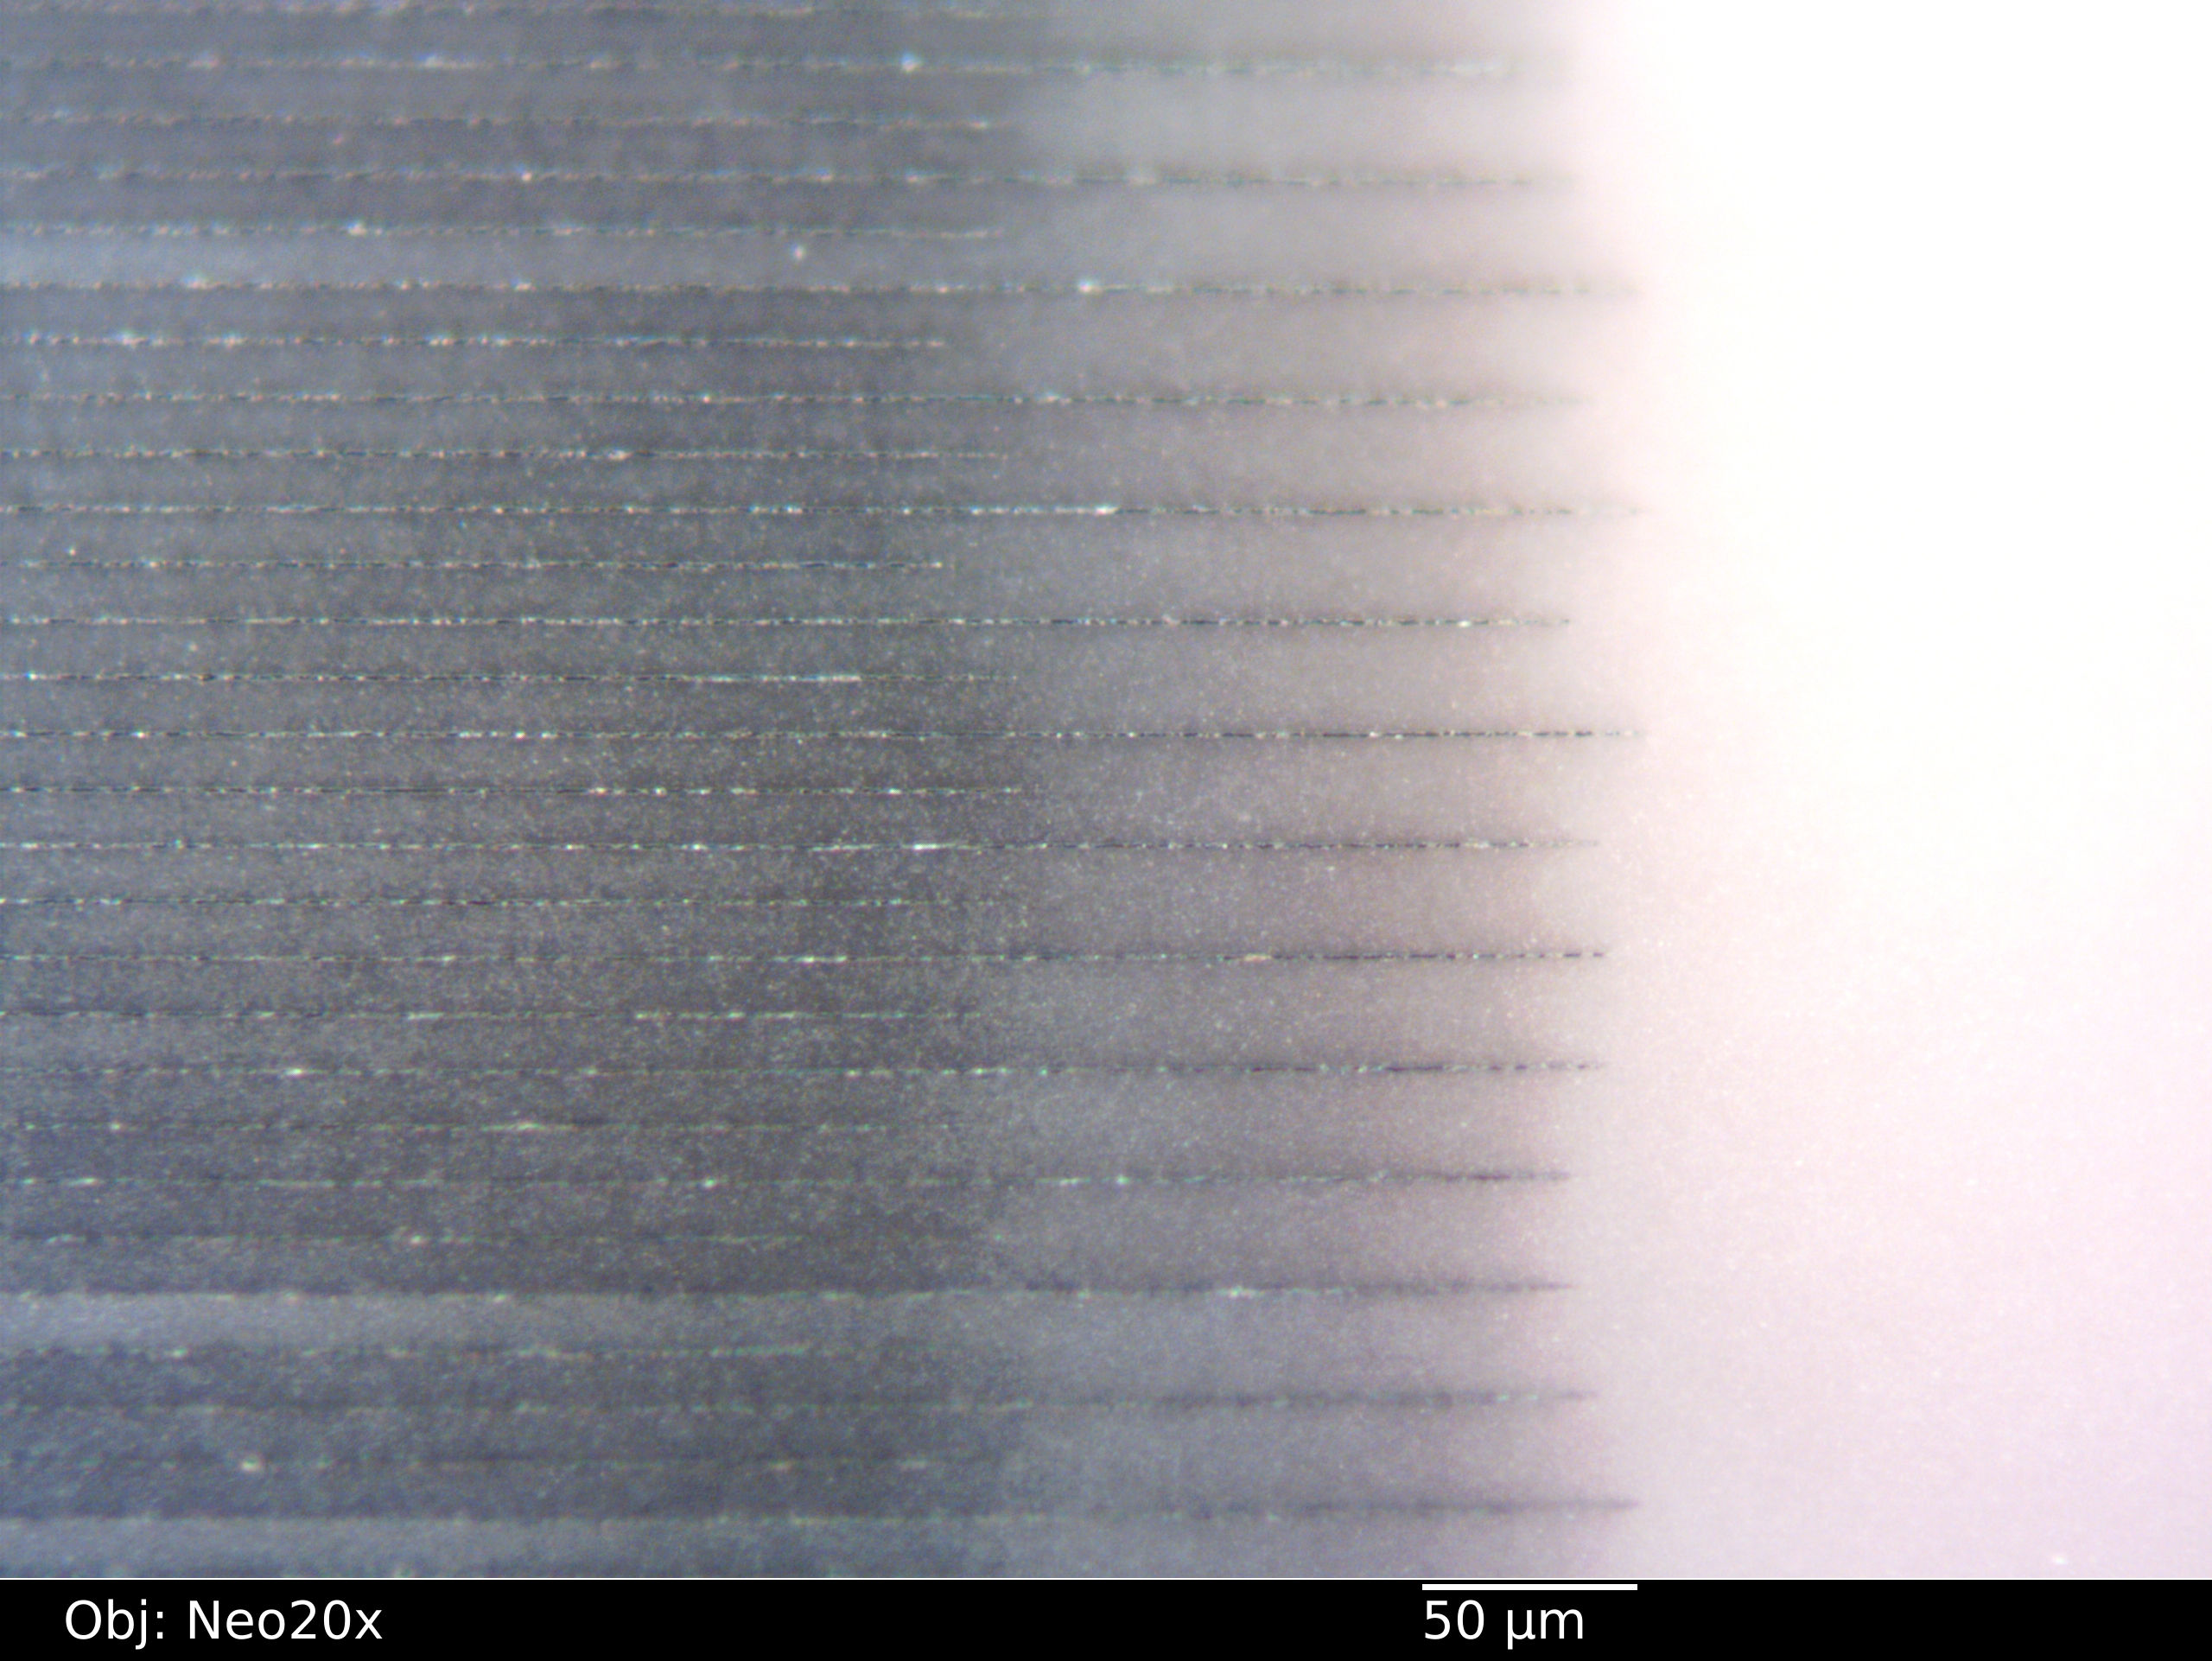
\includegraphics[width=11cm,keepaspectratio]{section2_05_df_neo20x_annotated.jpg}
\caption{Geometry of even/odd capacitor plates}
\label{plate-geometry}
\end{figure}

\begin{figure}[h]
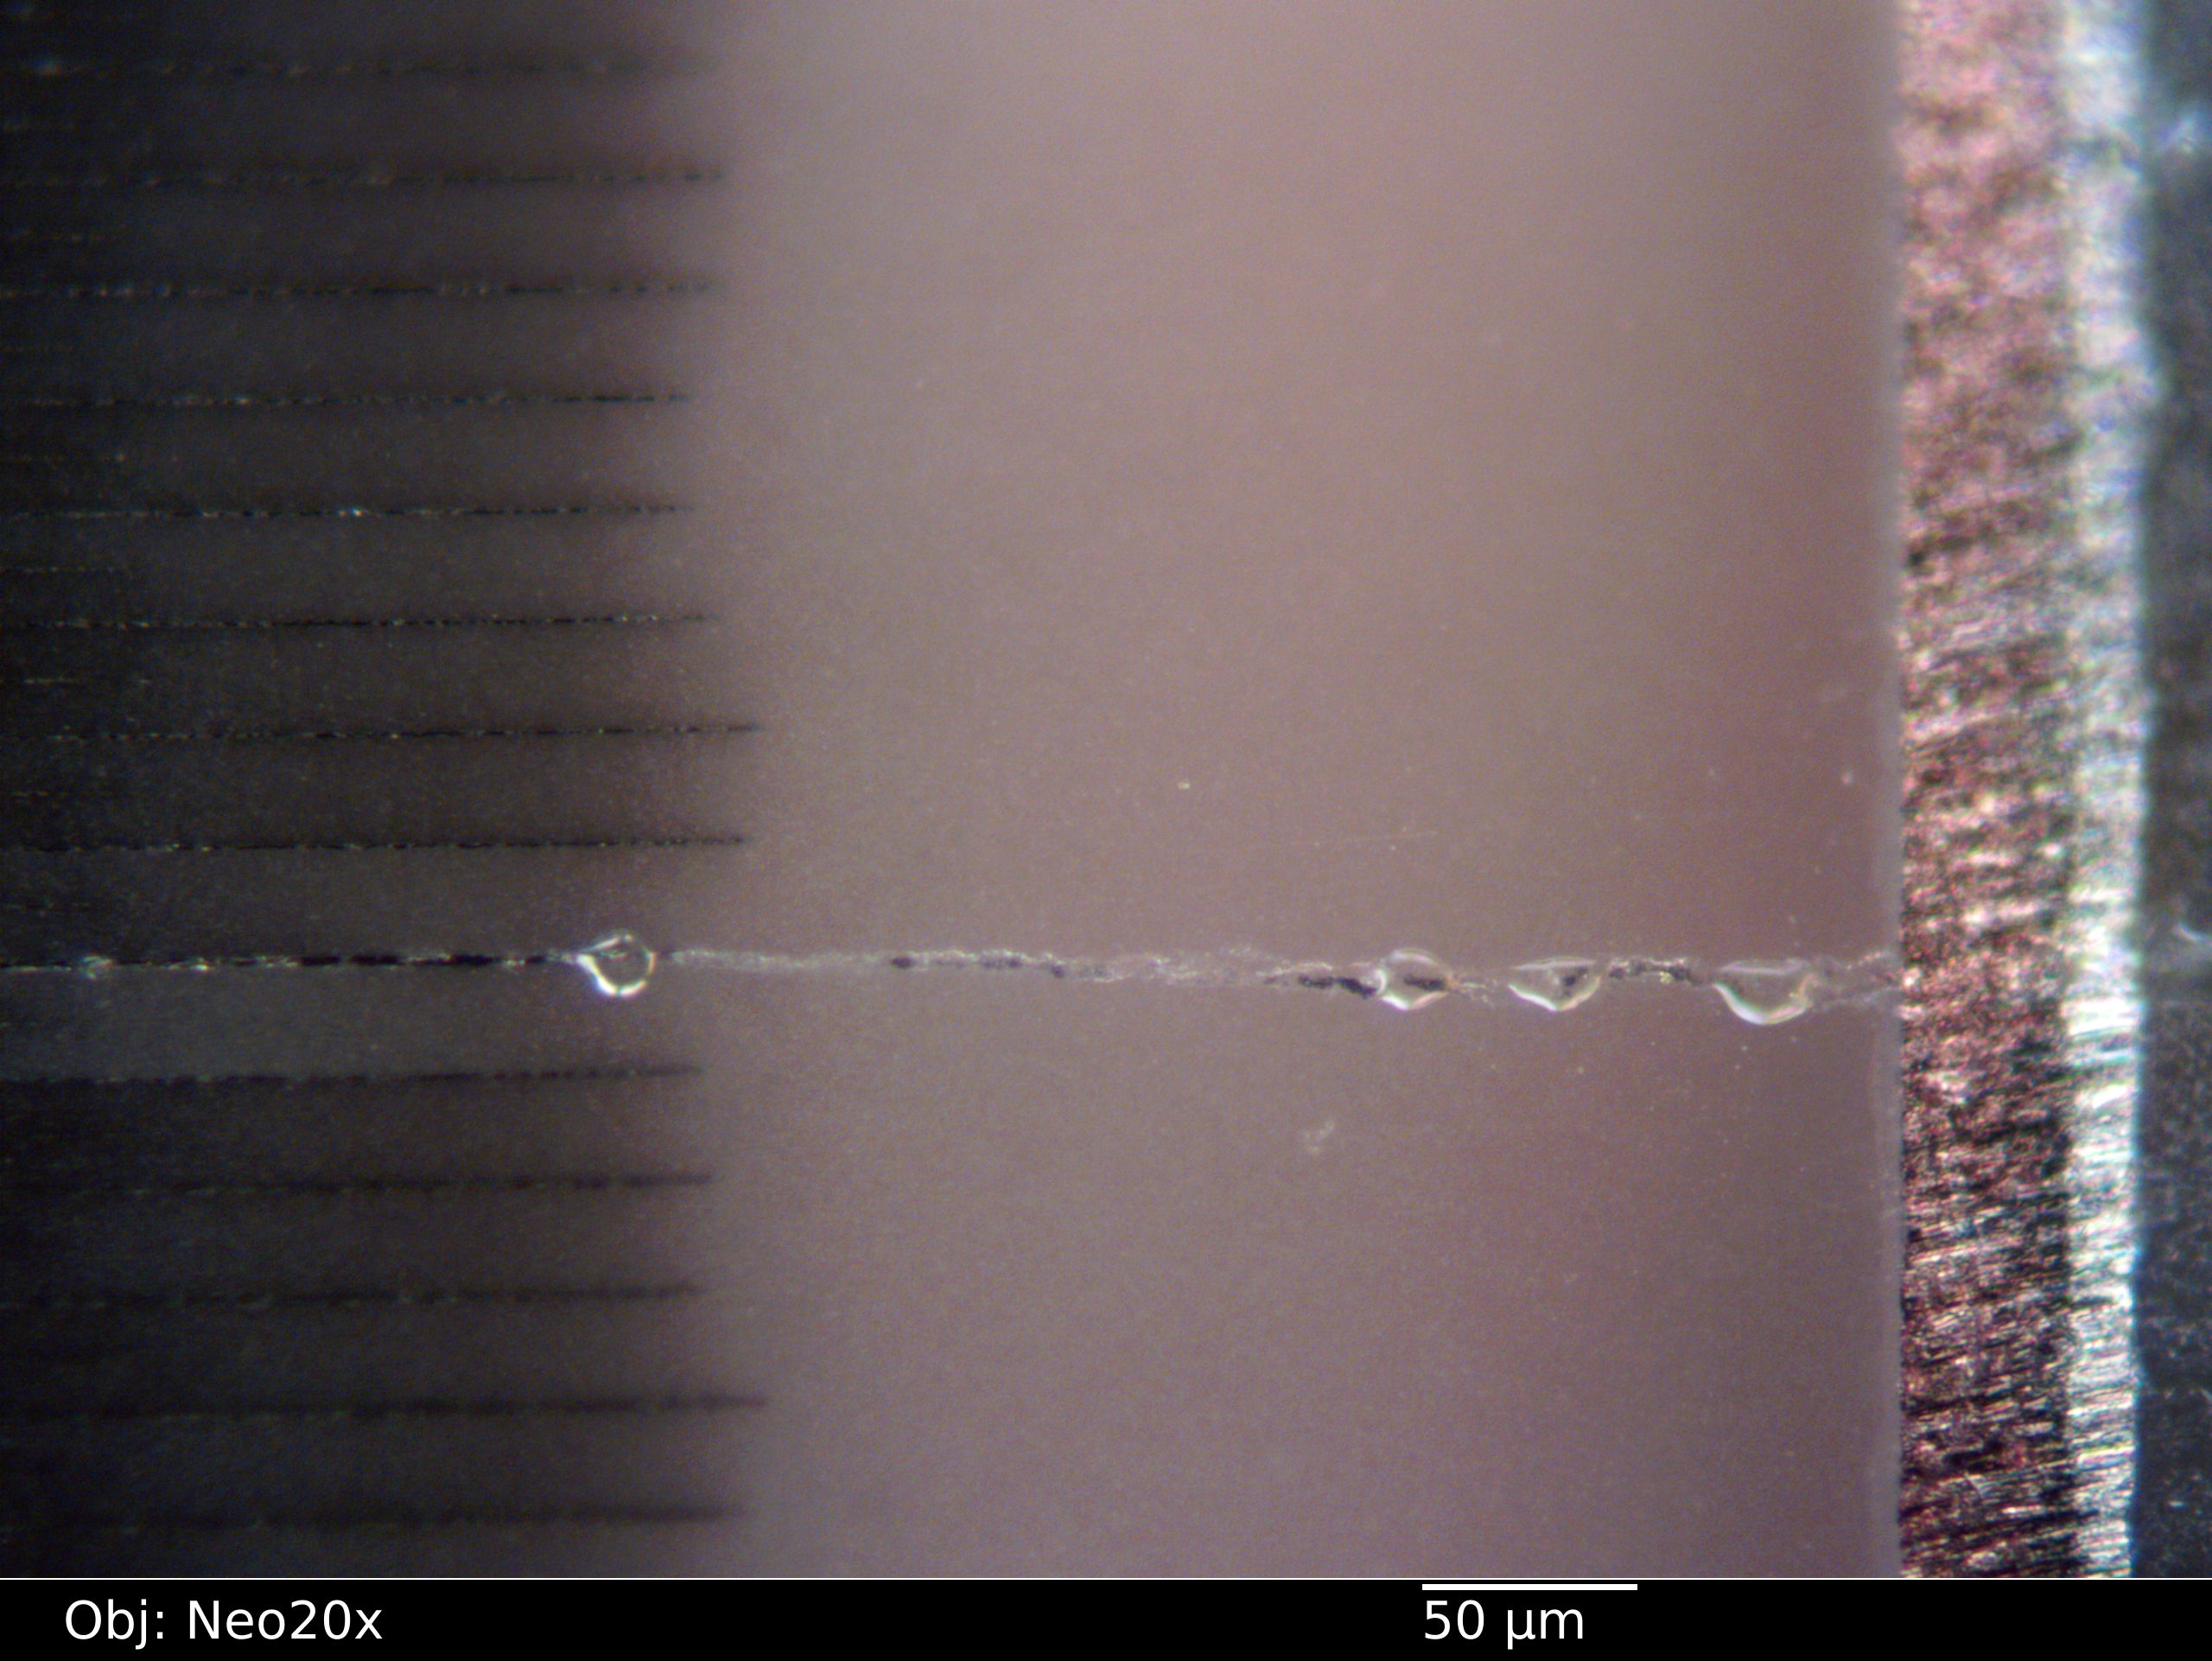
\includegraphics[width=11cm,keepaspectratio]{section2_07_df_neo20x_annotated.jpg}
\caption{Spalling around center plate, right side of plate stack}
\label{spalling}
\end{figure}

\begin{figure}[h]
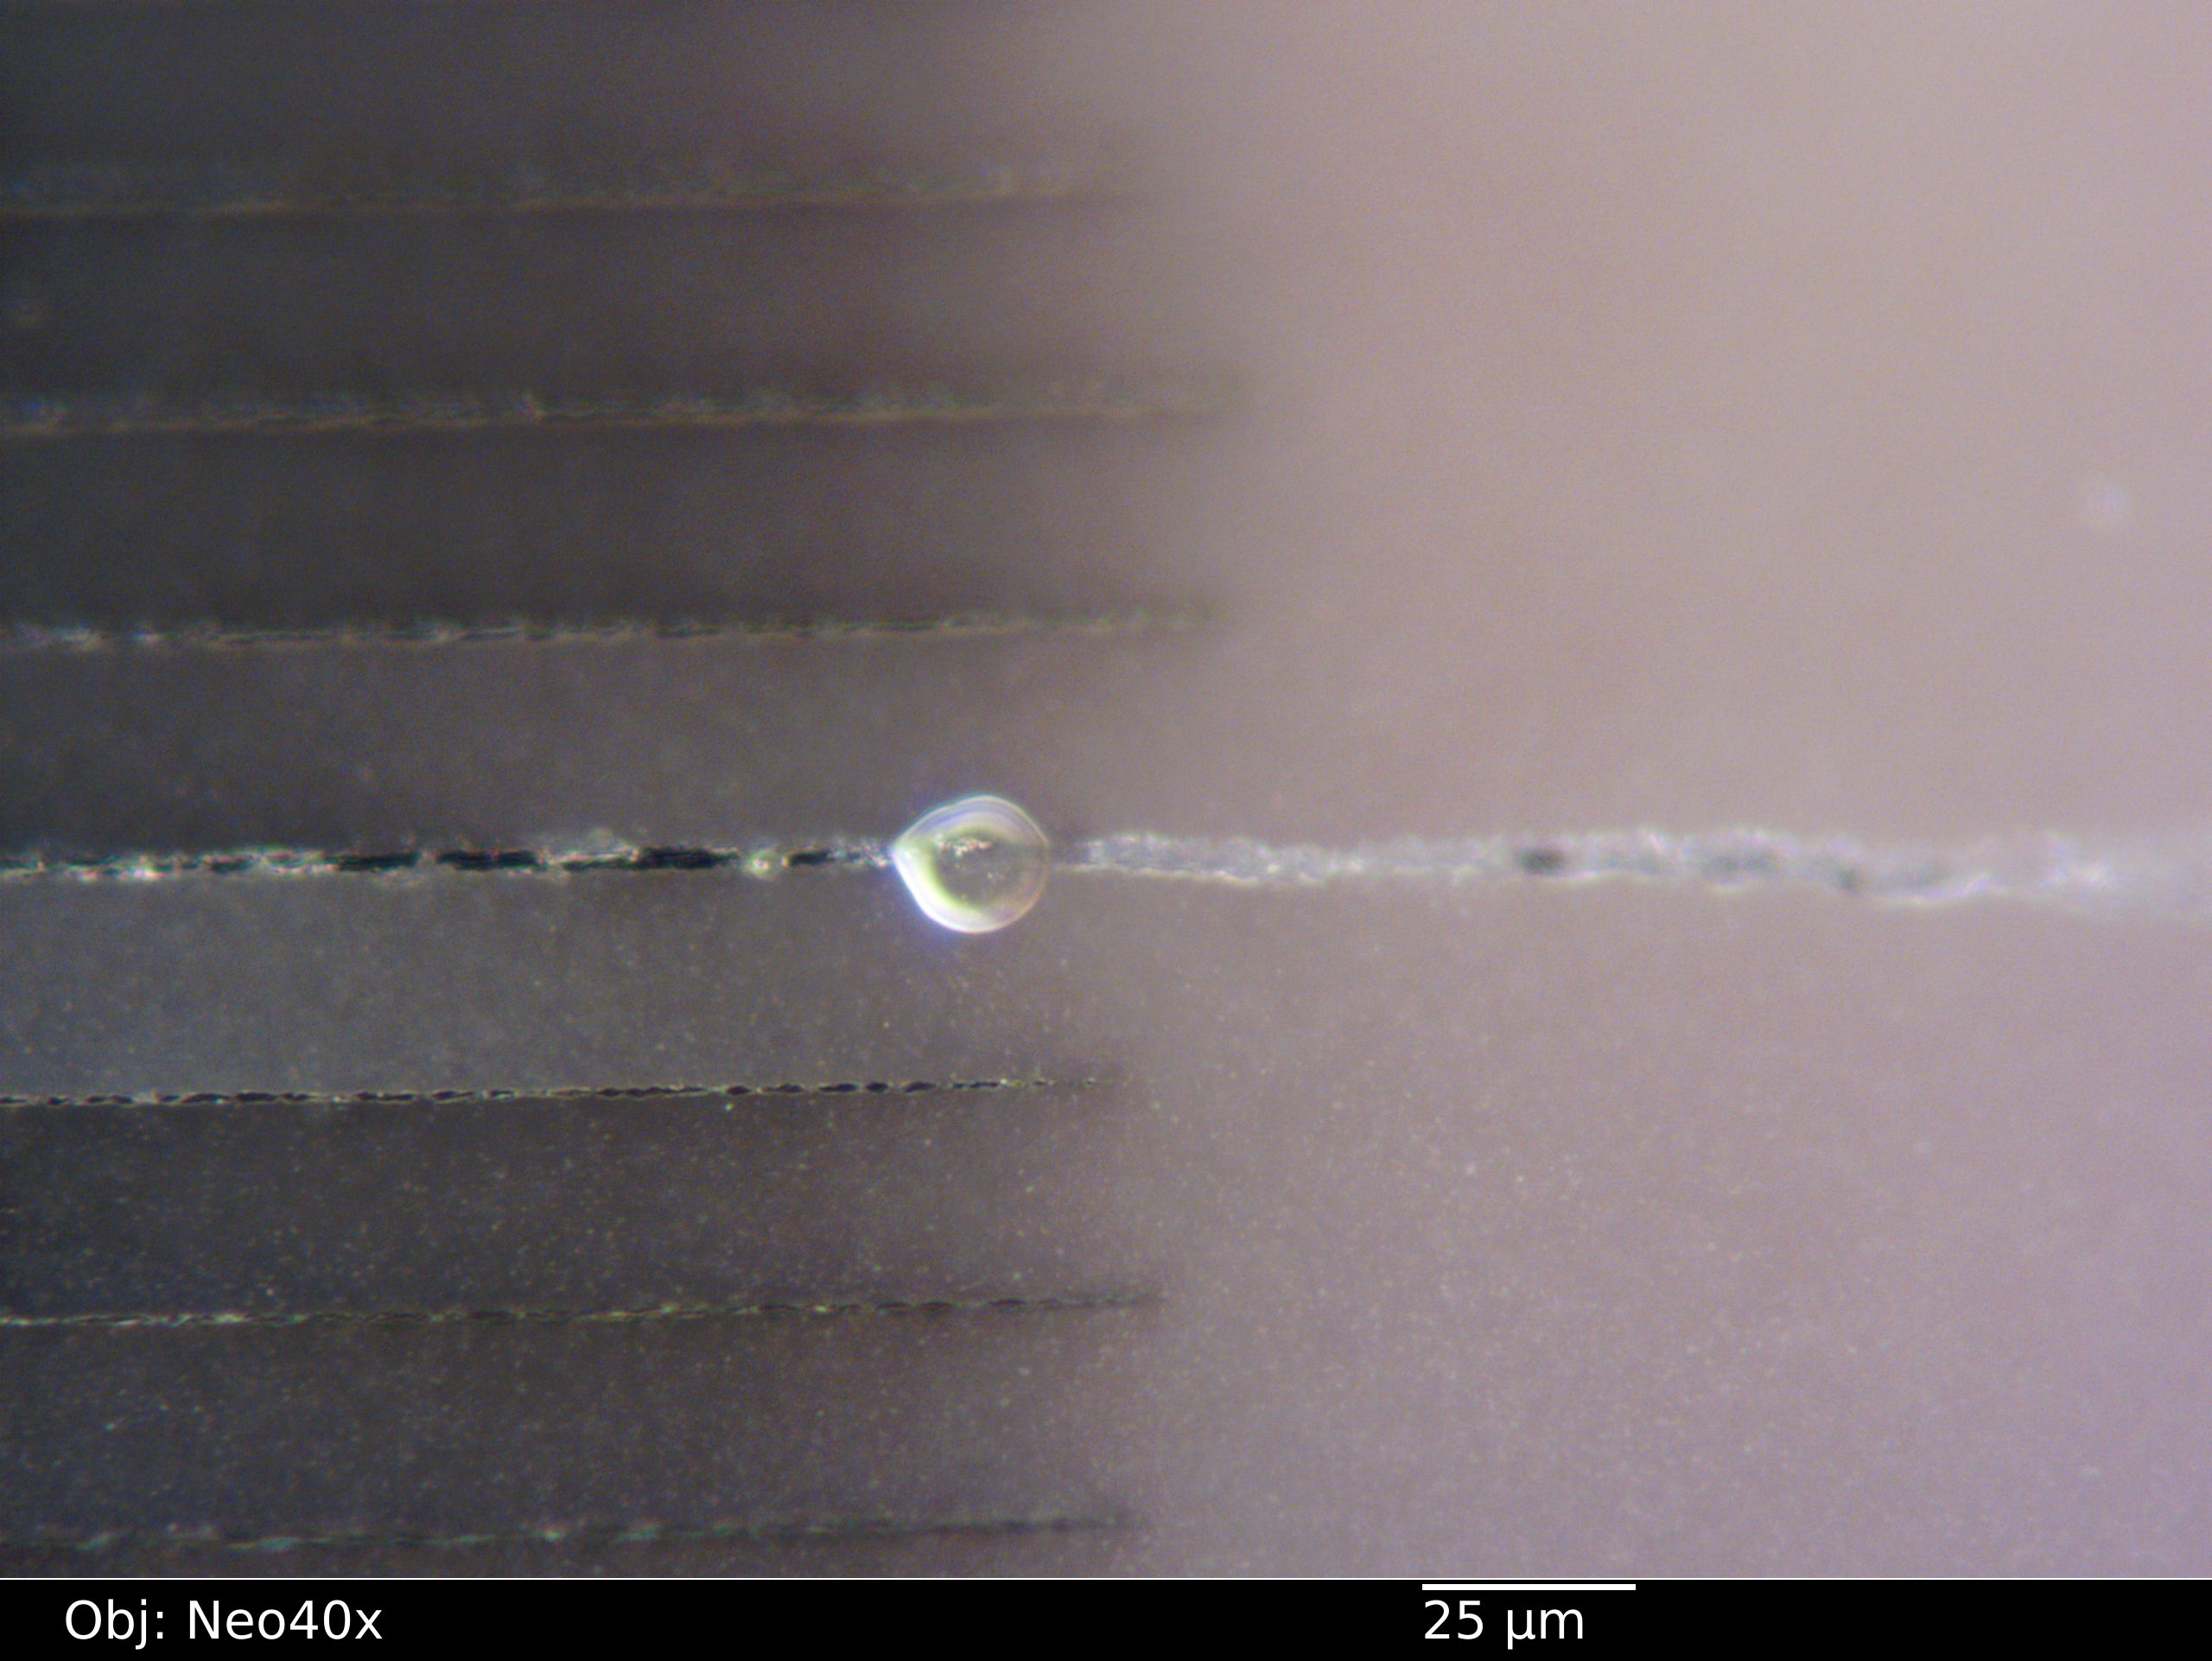
\includegraphics[width=11cm,keepaspectratio]{section2_09_bf_neo40x_annotated.jpg}
\caption{Spalling around center plate, right side of plate stack}
\label{spalling2}
\end{figure}

\begin{figure}[h]
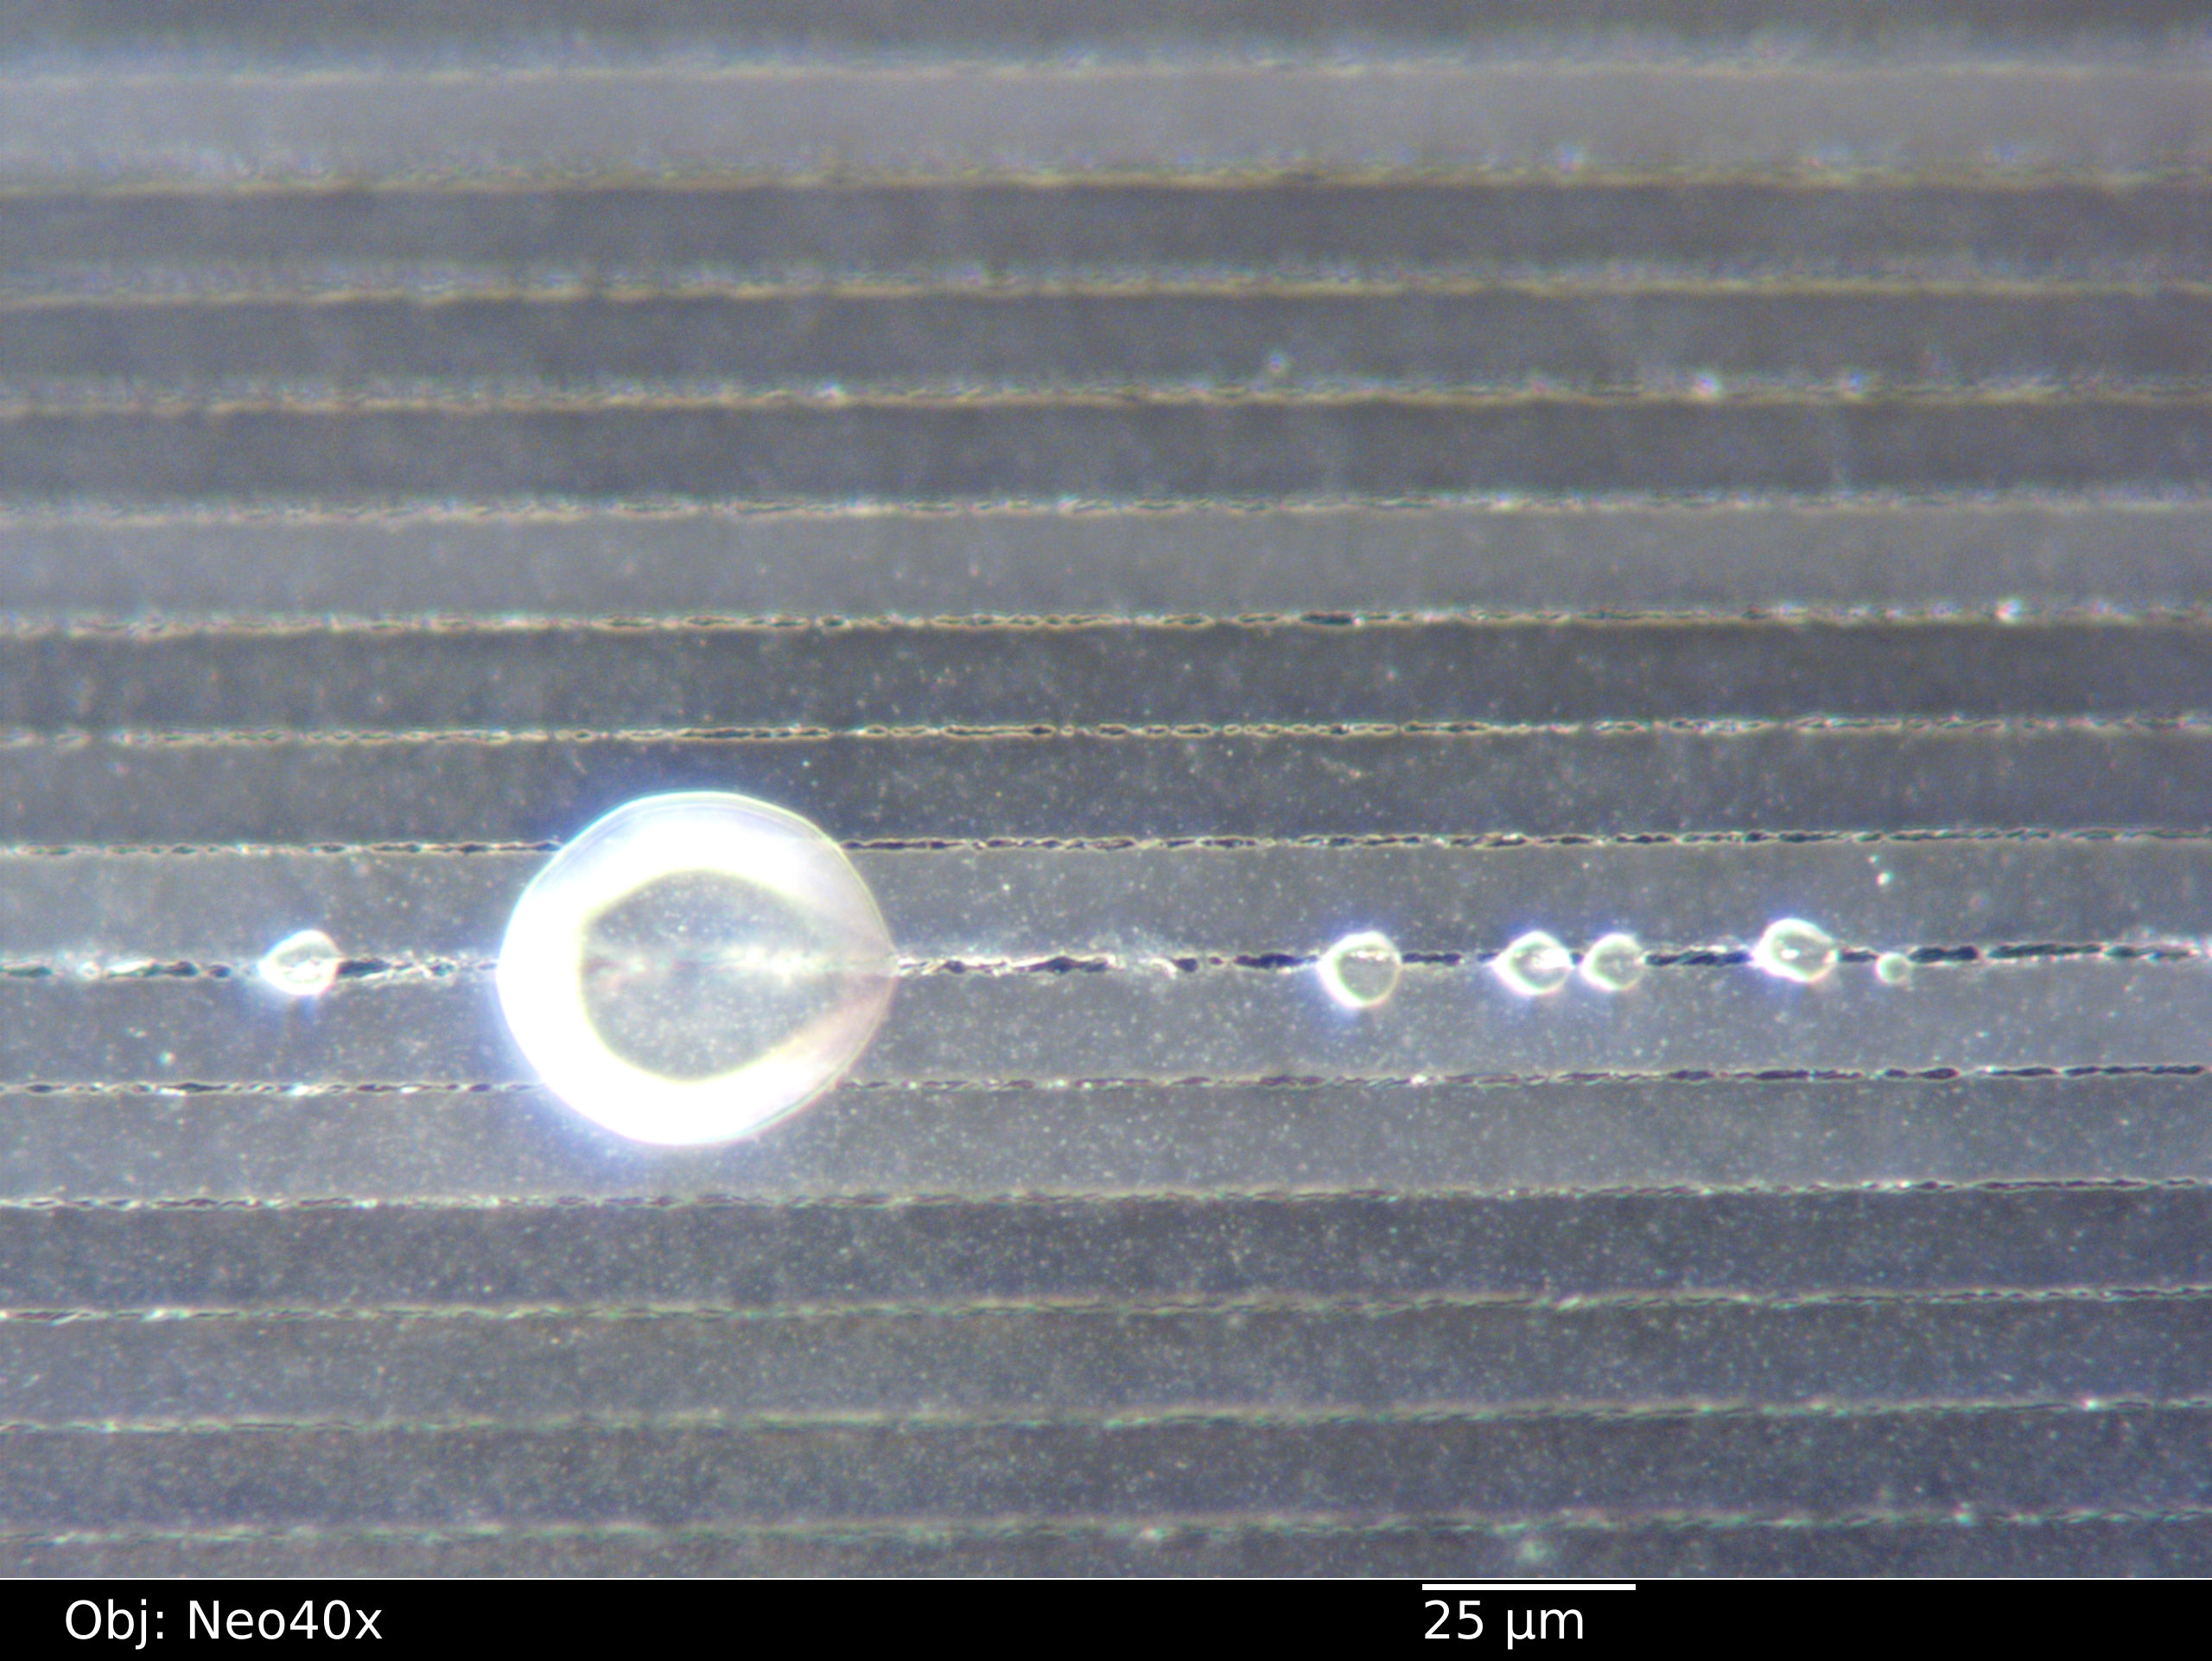
\includegraphics[width=11cm,keepaspectratio]{section2_10_df_neo40x_annotated.jpg}
\caption{Spalling around center plate, center of plate stack}
\label{spalling3}
\end{figure}

\FloatBarrier
\subsection{Slice 3}
The sample was ground down by an additional $100 \mu m$. No findings of note were observed in this section.

\subsection{Slice 4}

\end{document}
